\documentclass[main.tex]{subfiles}
\begin{document}
\glsresetall

\section{Introduction}

The \gls{cta} \cite{CTA} is the next generation observatory for ground-based for $\gamma$-ray astronomy. It is the result of the combination of efforts from all the $\gamma$-ray community, to push the field of \gls{vhe} astrophysics to new limits. It will consist on two arrays of \glspl{iact} located in the Northern hemisphere, in the Roque de los Muchachos Observatory in the island of La Palma (Canary Islands, Spain) and in the Southern hemisphere in the Paranal desert (Chile). With this configuration, \gls{cta} will be the first ground-based observatory to be able to observe the full sky. \gls{cta} will have five to ten times more sensitivity than current instruments in the broader energy range ever reached by \glspl{iact} facilities, from 20 GeV to 300 TeV. Its angular resolution down to to 2 arcseconds, with a field of view of $\sim 10º$ will allow the observation of fine structures in extended $\gamma$-ray sources. Its energy resolution, with an uncertainty less than 10\%, will make \gls{cta} able to study features in the sources spectra, such as lines and cutoffs, in great detail.\\
To reach such improvements with respect to the current generation of \glspl{iact} observatories, \gls{cta} will count with more than 100 telescopes in three sizes, each optimized for observation in a specific spectral range. \glspl{lst} have the bigger size, with a 32 m diameter mirror. They are optimal to observe the lowest part of the \gls{vhe} spectrum covered by \gls{cta} ($\sim$20 GeV to 3 TeV) where $\gamma$-rays are more abundant, so a small number of telescopes is enough, but the induced $\gamma$-ray showers emit a low number of Cherenkov photons, large mirrors are required to collect the maximum number of photons. \glspl{mst} have an intermediate size, with a diameter of$\sim 10$m. They have the best performance at the range between $\sim 100$ GeV and 50 TeV. \glspl{sst} have much smaller mirrors ($\sim$ 4 m), and a large number of them will be installed to get big collection areas and be able to capture the highest energy photons (up to 300 TeV), which are very rare but produce huge amounts of Cherenkov light.\\
Thanks to the large number of telescopes, \gls{cta} will have great flexibility of operations, with different observation modes: with full array for best sensitivity; using subarrays to observe several sources at the same time; and divergent pointing mode where the field of view can be extended up to 20 deg.\\
In this chapter the main features of \gls{cta} are covered. A description of performance is given in section \ref{sec:ctaperformance}. In section \ref{sec:ctatelescopes} the three types of telescopes are described in detail. Section \ref{sec:ctaanalysis} is dedicated to \gls{cta} data analysis techniques and tools at different levels.

\section{CTA Requirements and Performance} \label{sec:ctaperformance}

The current generation of Cherenkov telescope observatories consist on arrays of 2 to 5 telescopes which reach sensitivities of about 1\% of the Crab flux at the range of 0.1-1 TeV for 50h observation time. Their typical angular resolution is about 0.1º, but it can reach 0.02º for intense point sources of 20 to 30 arc seconds. The goal of \gls{cta} design is to advance the state of the art in $\gamma$-ray astronomy, improving sensitivity, energy range, angular and timing resolution and offering full sky coverage. The performance goals of \gls{cta} are shown in table \ref{tab:CTAgoals}. As a consequence of these goals, \gls{cta} will provide for two unique features: the ability to produce a deep survey of the \gls{vhe} sky, potentially discovering hundreds of new sources; and the possibility to observe short time-scale phenomena, such as flares and jets from black holes in the center of active galaxies or periodic emission like such of pulsars. 
To achieve these improvements with respect to current \gls{iact} facilities, different types of telescopes are required and they should be spread over large areas to reach a collection area of several km$^2$ \cite{CTAconcept}.

\begin{table}
  \centering
  \begin{tabular}{ccc}
    \hline
    Diff. sensitivity & at 50 GeV & $8\times10^{-12}$\\
    (erg cm$^2$ s$^{-1}$) & at 1 TeV & $2\times10^{-13}$\\
     & at 50 TeV & $3\times10^{-13}$ (S) / $3\times10^{-12}$ (N)\\\\
    Collection area (m$^{2}$) & at 1 TeV & > $10^4$ \\
    & at 10 TeV & > $10^6$ (S)/ >$5\times10^5$ (N) \\\\
    Angular resolution & at 0.1 TeV & 0.1º \\
    & > 1 TeV & 0.05º \\\\
    Energy resolution & at 50 GeV & $\le 25\%$ \\
    & > 1 TeV & $\le 10\%$ \\\\
    Field of view & at 0.1 TeV & 5º\\
    & at 1 TeV & 8º\\
    & > 10 TeV & 10º\\\\
    Sensitivity in FoV & at 1 TeV flat out to & > 2.5º \\
    & at 1 TeV & 5'' per axis \\\\
    Repointing time & <0.1 TeV  & 20s (goal), 50s(max) \\
    & 0.1-10 TeV & 60s (goal), 90s (max) \\
    \hline
  \end{tabular}
  \caption{Performance goals for CTA observatories, adapted from \cite{CTAconcept}. Sensitivity given in 5 bins per energy. (N)= Northern site, (S) = Southern site.}
  \label{tab:CTAgoals}
\end{table}

The final performance of \gls{cta} depends on the design of the telescopes, which will be discussed more deeply in next sections, and also on the arrangement of them in the two sites.
To optimize the observatory configuration and estimate its performance,  detailed Monte Carlo simulations were made \cite{2013CTAMonteCarlo}, comprising simulations of shower development in the atmosphere, detector response and event reconstruction.
A deep study of these simulations \cite{2017CTAMCPerformance} for different configurations of telescopes and sites came up with the final array layout illustrated in picture \ref{fig:arraylayout}.

\begin{figure}
\centering
 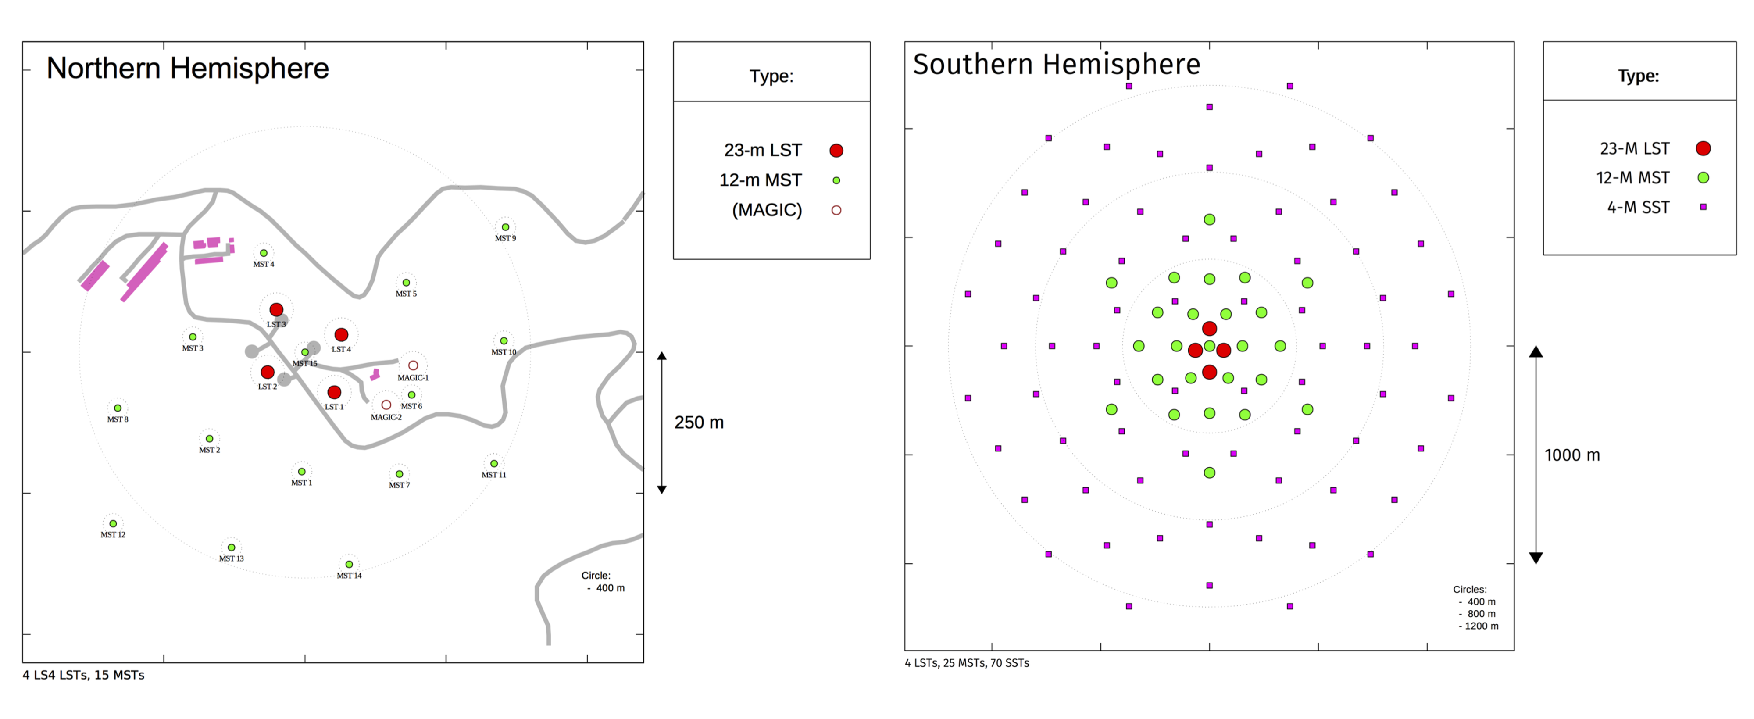
\includegraphics[width=1\textwidth]{Pictures/Array-Layouts.pdf}
  \caption{Array layout selected for \gls{cta} from \cite{CTAPerformance}. Left is Northern site where also \gls{magic} telescopes are located. Right is Southern location.}
    \label{fig:arraylayout}
\end{figure}

The baseline design for Southern observatory foresees 4 \glspl{lst}, 25 \glspl{mst} and 70 \glspl{sst}. It will be dedicated to the study of galactic sources which emit the most energetic $\gamma$-rays that can reach the Earth. Because of their extremely low fluxes, it will cover very a large area ($\sim4$ km$^2$), achieved thanks to the large number of \glspl{sst}, to capture as many events as possible.\\
The Northern observatory will mainly observe extragalactic sources and transient events from which only the less energetic photons reach the Earth due to absorption (see section \ref{sec:absorption}). Its final configuration will consist on 4 \glspl{lst} and 15 \glspl{mst}.

The performance of \gls{cta} has been evaluated for the observation of a point source located at the centre of the field of view of telescopes cameras. A set of metrics are taken into account: Effective collection area, residual cosmic-ray background rate, angular resolution and differential sensitivity. Usually they are calculated after applying $\gamma$-hadron separation cuts, using the quantities \textit{gammaness} and $\theta^2$ (defined in section \ref{sec:IACTs}), optimized to maximize the sensitivity for a set of typical observation times.
An overview of the mentioned metrics for performance evaluation is the following:\\

\begin{itemize}
\item \textbf{Effective collection area:} The effective collection area describes the area of the upper atmosphere were an incident $\gamma$-ray would be detected if \gls{cta} would have a detection efficiency, after cuts, of 100\%. The effective collection areasfor the assumed point sources are shown in figure \ref{fig:effarea}.\\

\begin{figure}[!htb]
\minipage{0.5\textwidth}
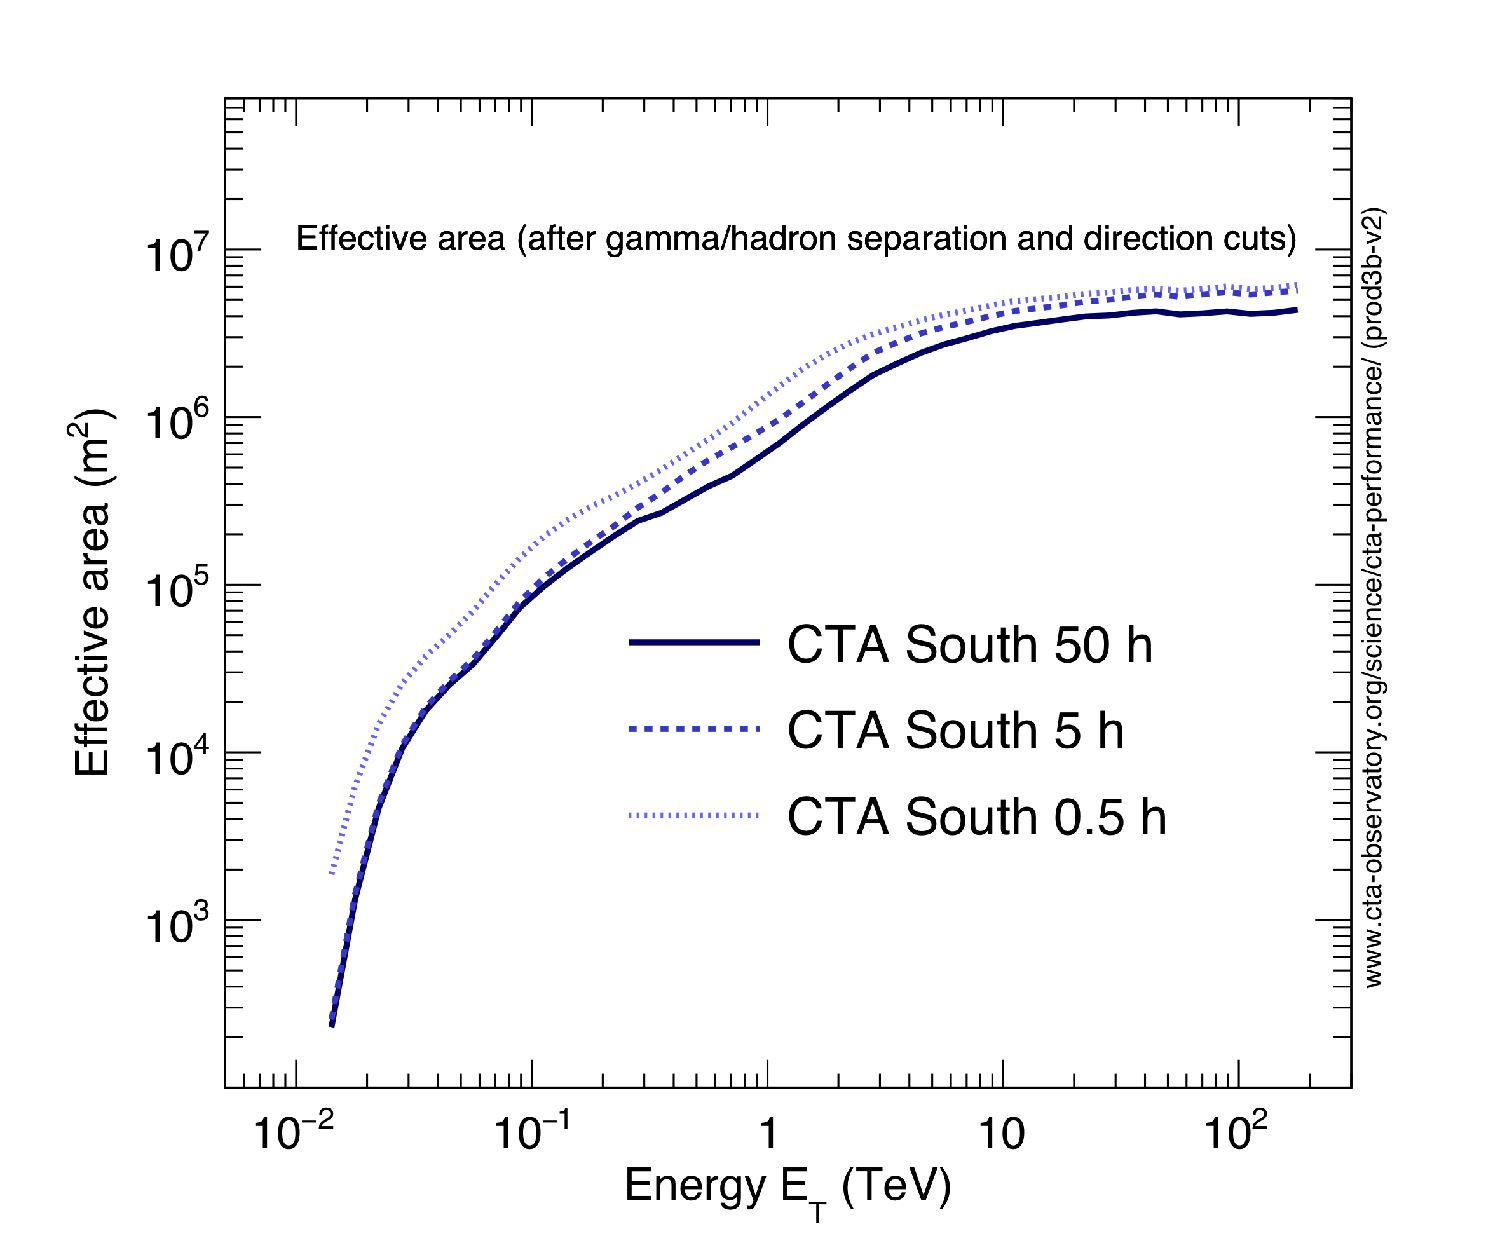
\includegraphics[width=\linewidth]{Pictures/CTA-Performance-prod3b-v2-South-20deg-EffectiveArea.pdf}
\endminipage\hfill
\minipage{0.5\textwidth}
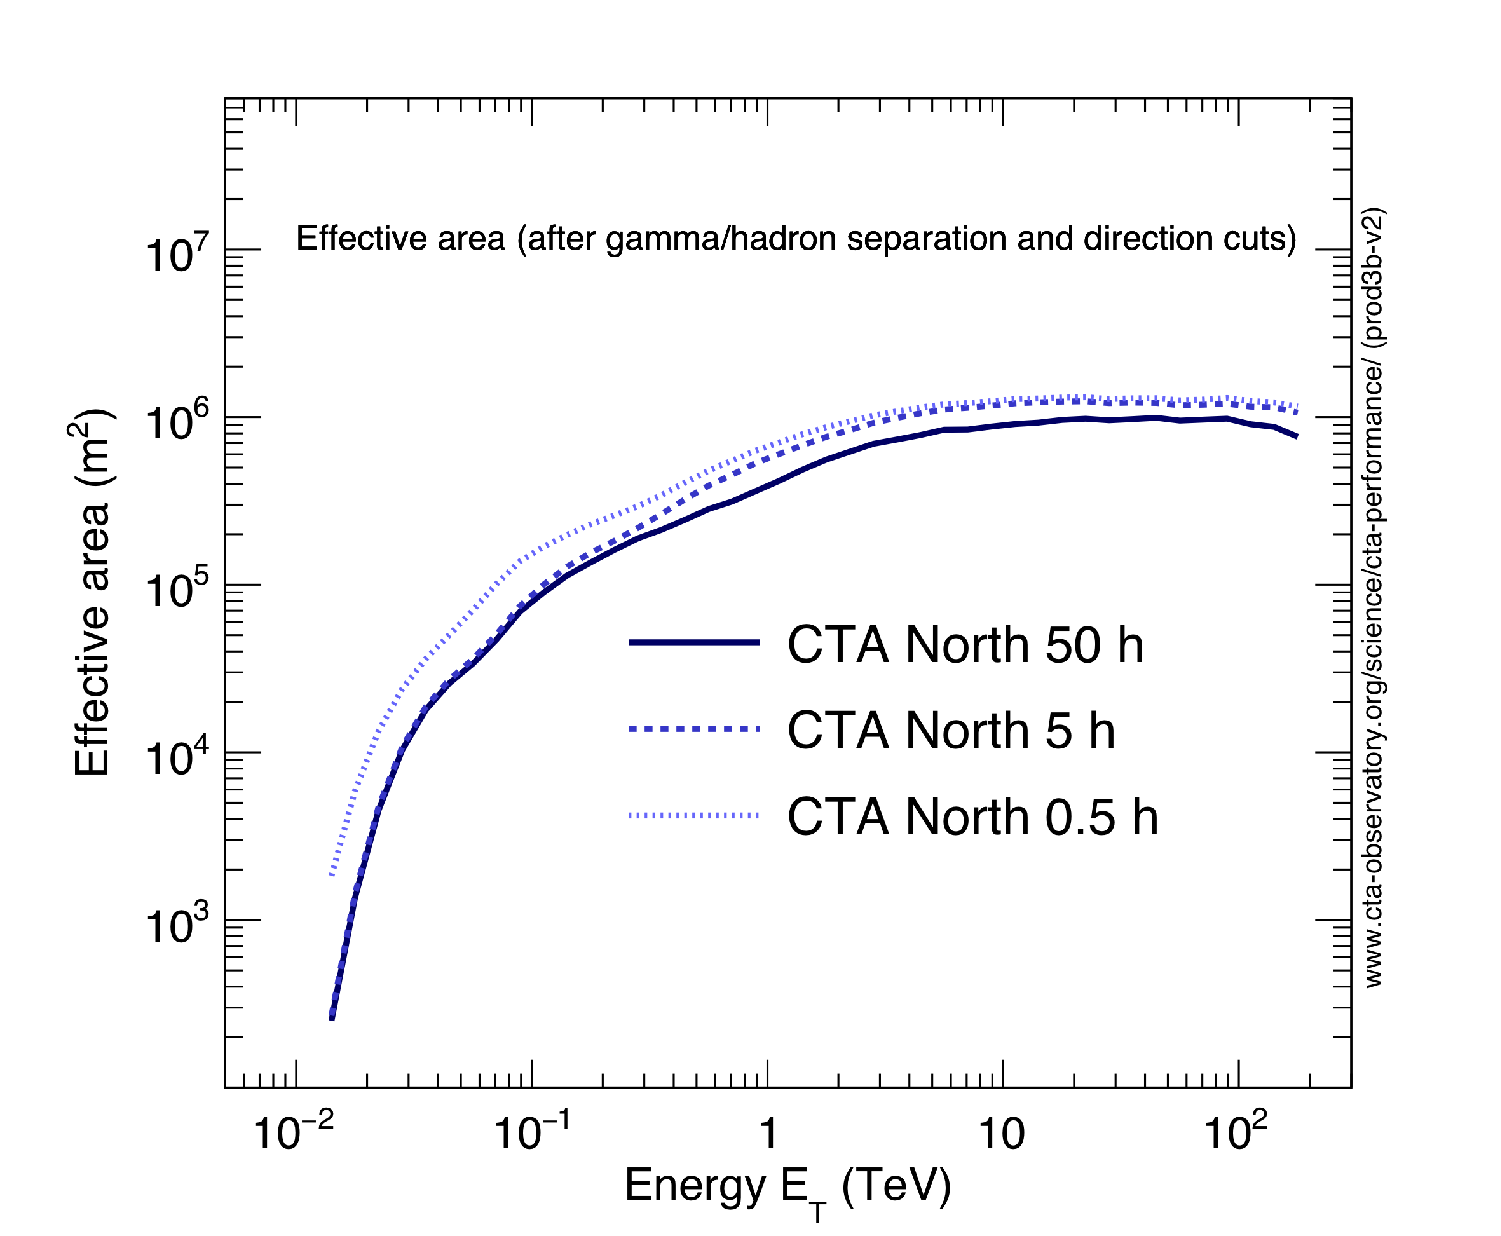
\includegraphics[width=\linewidth]{Pictures/CTA-Performance-prod3b-v2-North-20deg-EffectiveArea.pdf}
\endminipage\hfill
\caption{\label{fig:effarea}Effective collection area for point-like sources for CTA South(left) and CTA North (right) \cite{CTAPerformance}.}
\end{figure}

\item \textbf{Residual cosmic-ray background rate:} The ability of \gls{cta} to reject background events due to showers produced by \glspl{cr} instead of $\gamma$-rays is measured through the residual \gls{cr} background rate. 99.9\% of the showers reaching the telescopes are produced by \glspl{cr}, so a good background rejection is mandatory for \glspl{iact}. In figure \ref{fig:bkgrate} the post-analysis resulting cosmic-ray background rate per square degree vs reconstructed $\gamma$-ray energy is shown. The rate is integrated in each bin, where five bins per decade has been taken. \gls{cta} background rejection capabilities allow to reject the majority of the background in the range 0.2-1.5 TeV, where the remaining background is due to cosmic-ray electrons and positrons \cite{2017ICRCCTAPerformance} which produce showers very similar to those produced by $\gamma$-rays (see section \ref{sec:electroshowers}), making them an irreducible background.\\

  \begin{figure}[!htb]
    \minipage{0.5\textwidth}
    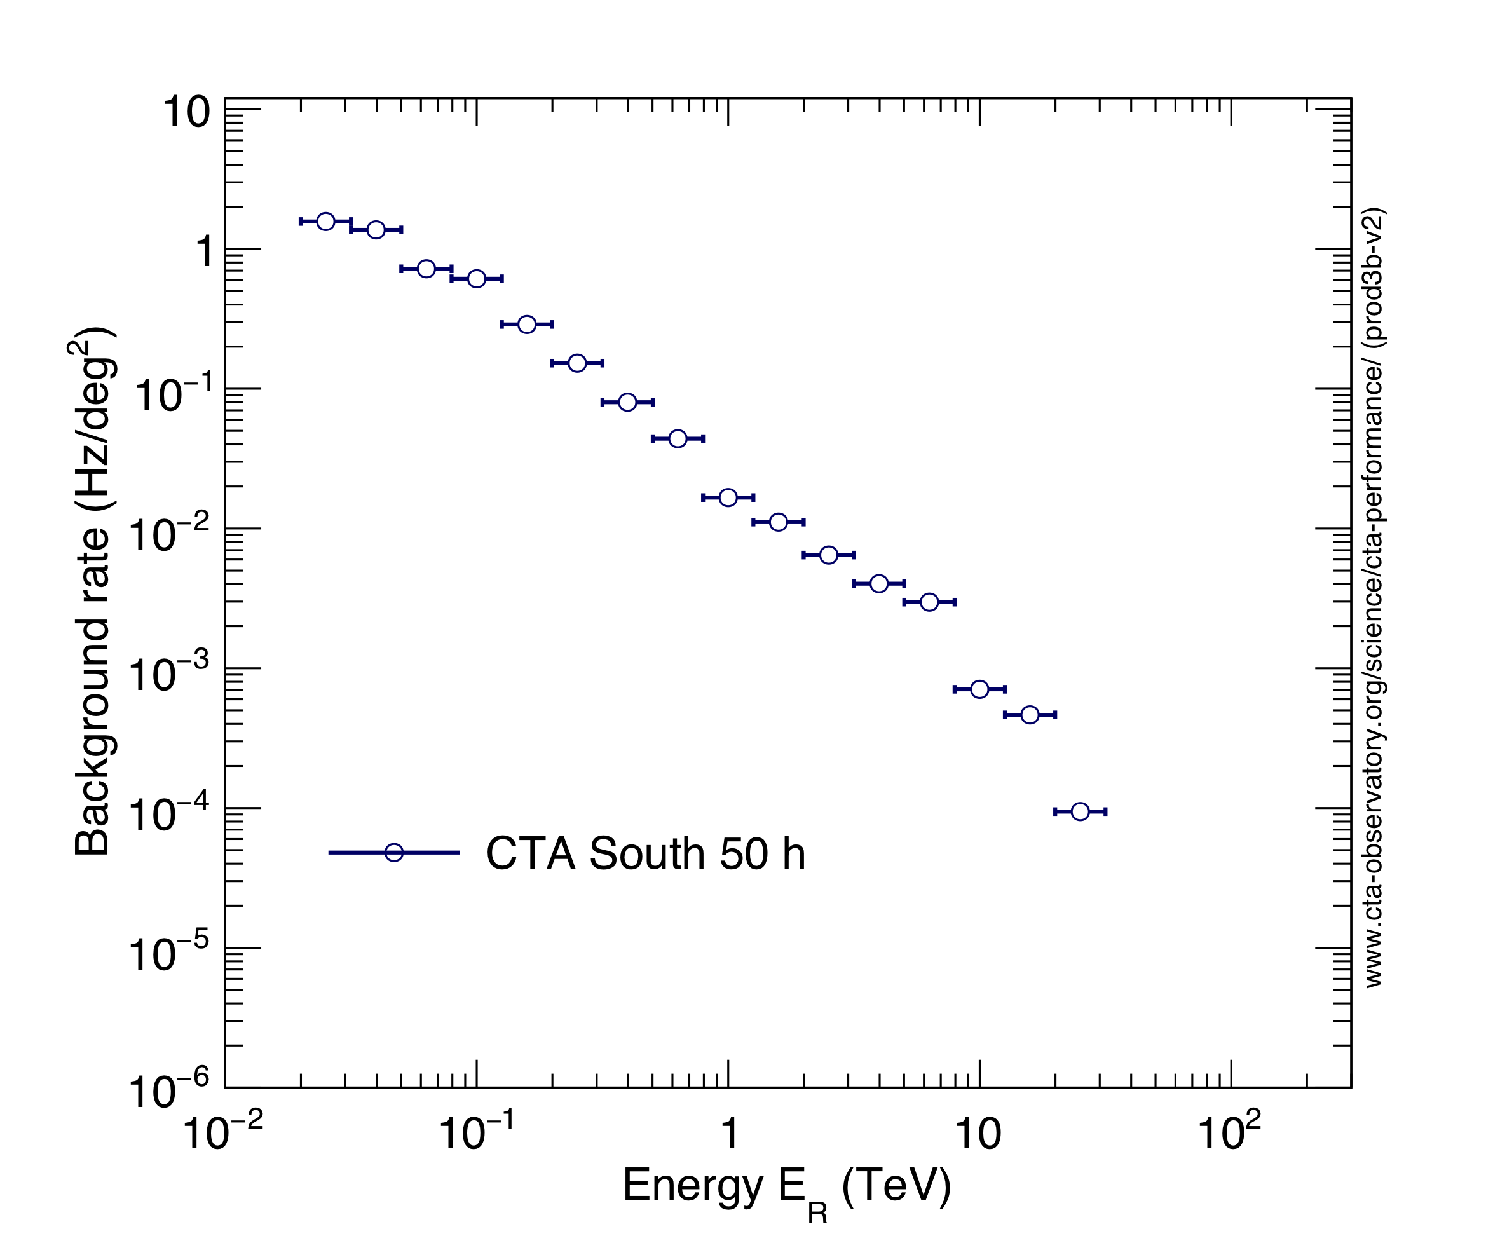
\includegraphics[width=\linewidth]{Pictures/CTA-Performance-prod3b-v2-South-20deg-BackgroundRateSquDeg.pdf}
    \endminipage\hfill
    \minipage{0.5\textwidth}
    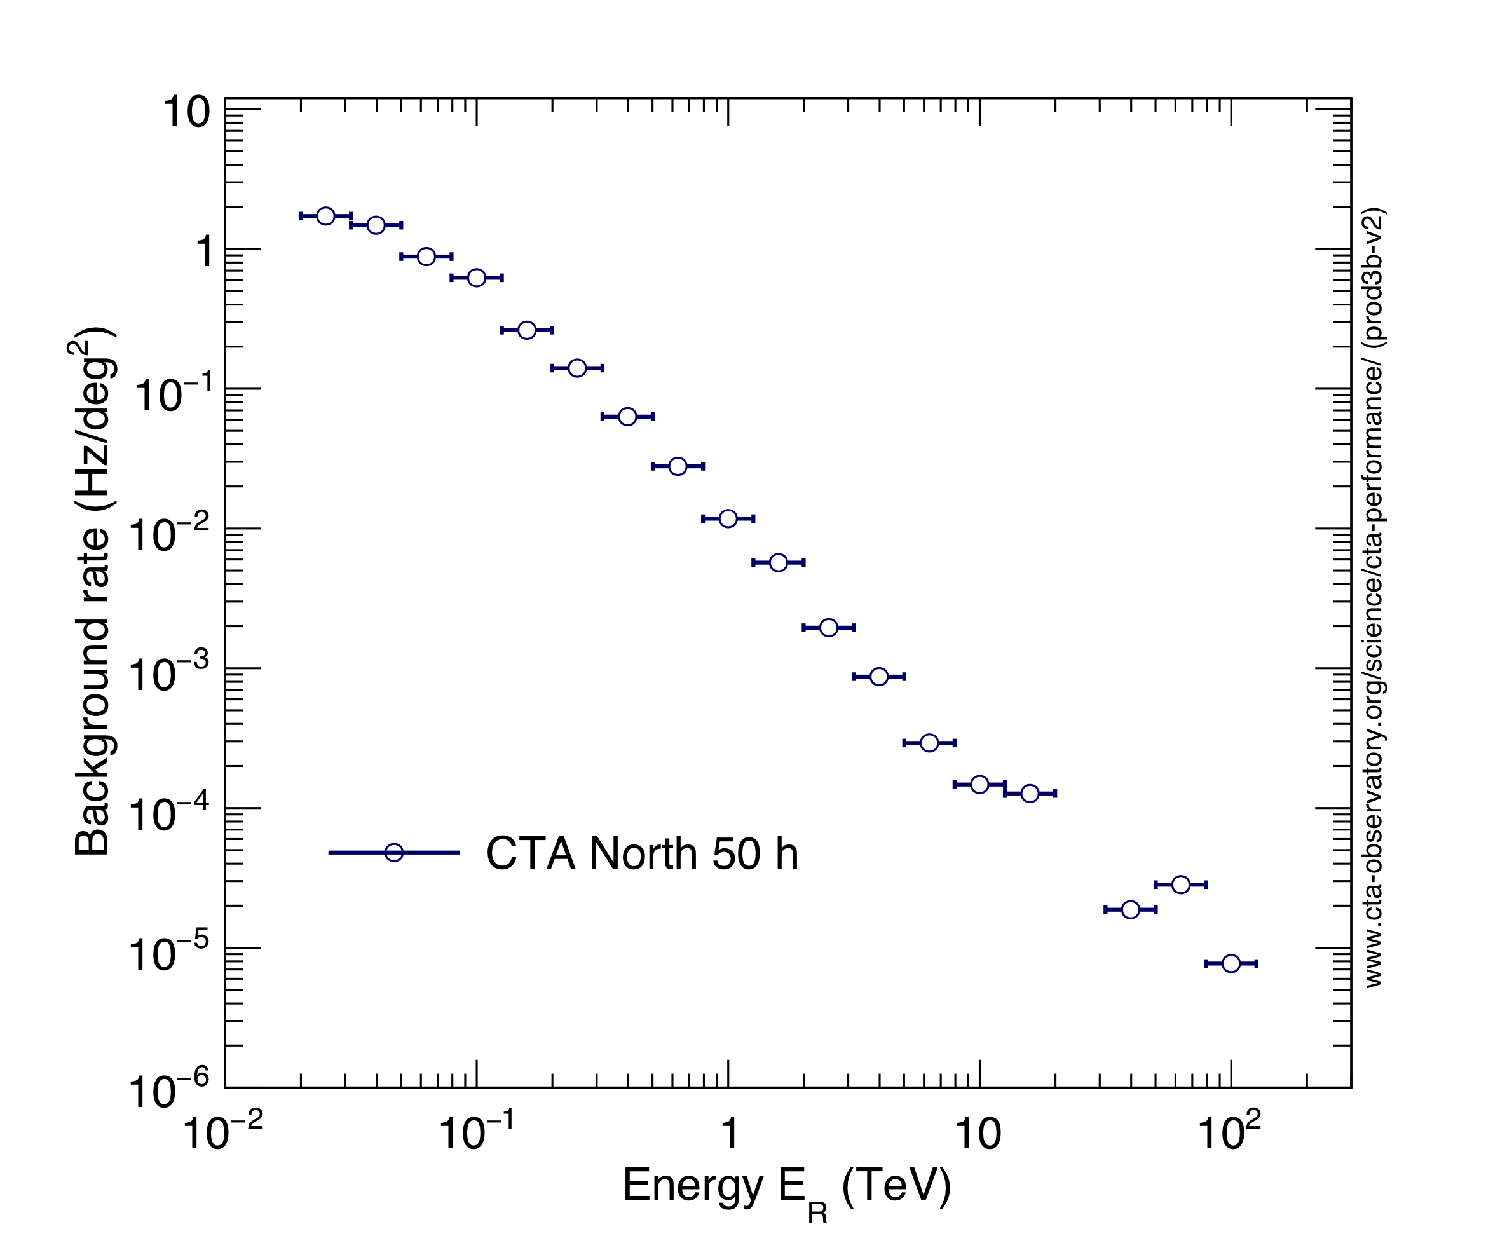
\includegraphics[width=\linewidth]{Pictures/CTA-Performance-prod3b-v2-North-20deg-BackgroundRateSquDeg.pdf}
    \endminipage\hfill
    \caption{\label{fig:bkgrate} Residual cosmic-ray background rate vs reconstructed energy for CTA South(left) and CTA North (right) \cite{CTAPerformance}.}
  \end{figure}
  
\item \textbf{Angular resolution:} The angular resolution is defined as the angle within which 68\% of reconstructed $\gamma$-rays fall, relative to their true direction. Figure \ref{fig:angres} show the angular resolution vs. reconstructed energy optimized for best point-source sensitivity. It is possible to improve angular resolution at expenses of collection area for a better study of morphological features of bright sources.\\
  
  \begin{figure}[!htb]
    \minipage{0.5\textwidth}
    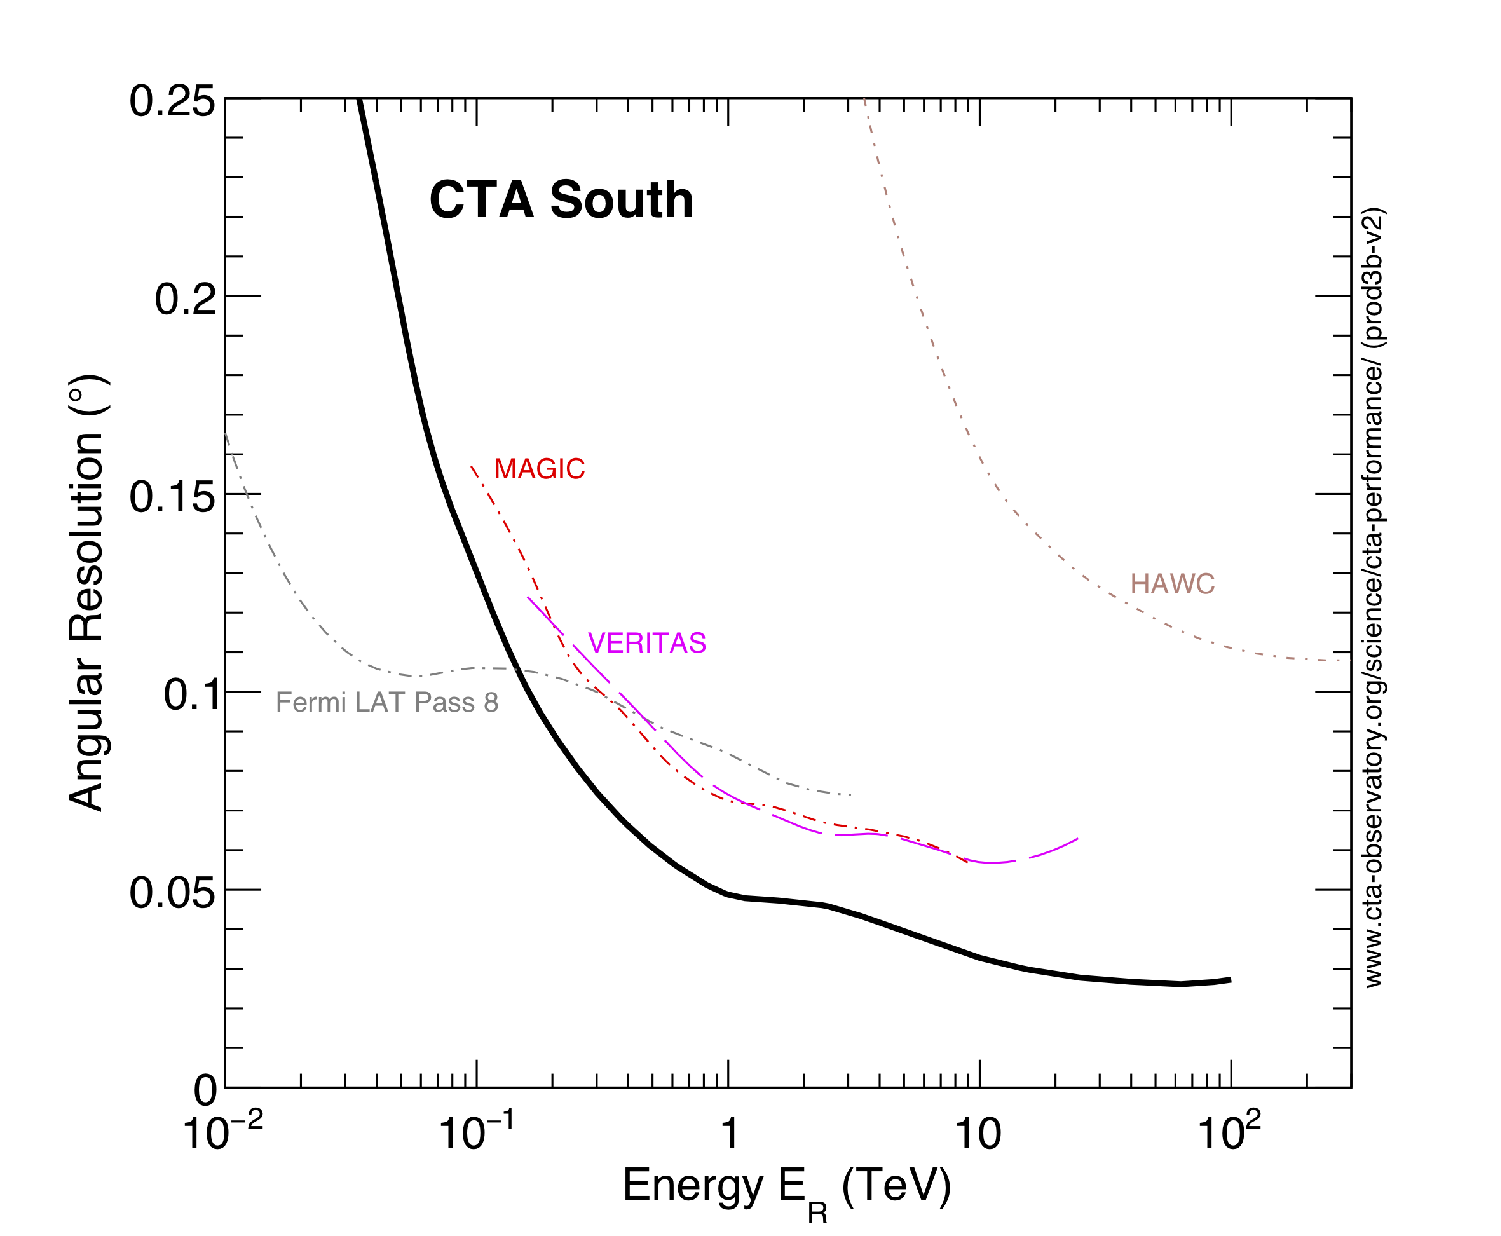
\includegraphics[width=\linewidth]{Pictures/CTA-Performance-prod3b-v2-Comparison-AngularResolution-OtherInstruments.pdf}
    \endminipage\hfill
    \minipage{0.5\textwidth}
    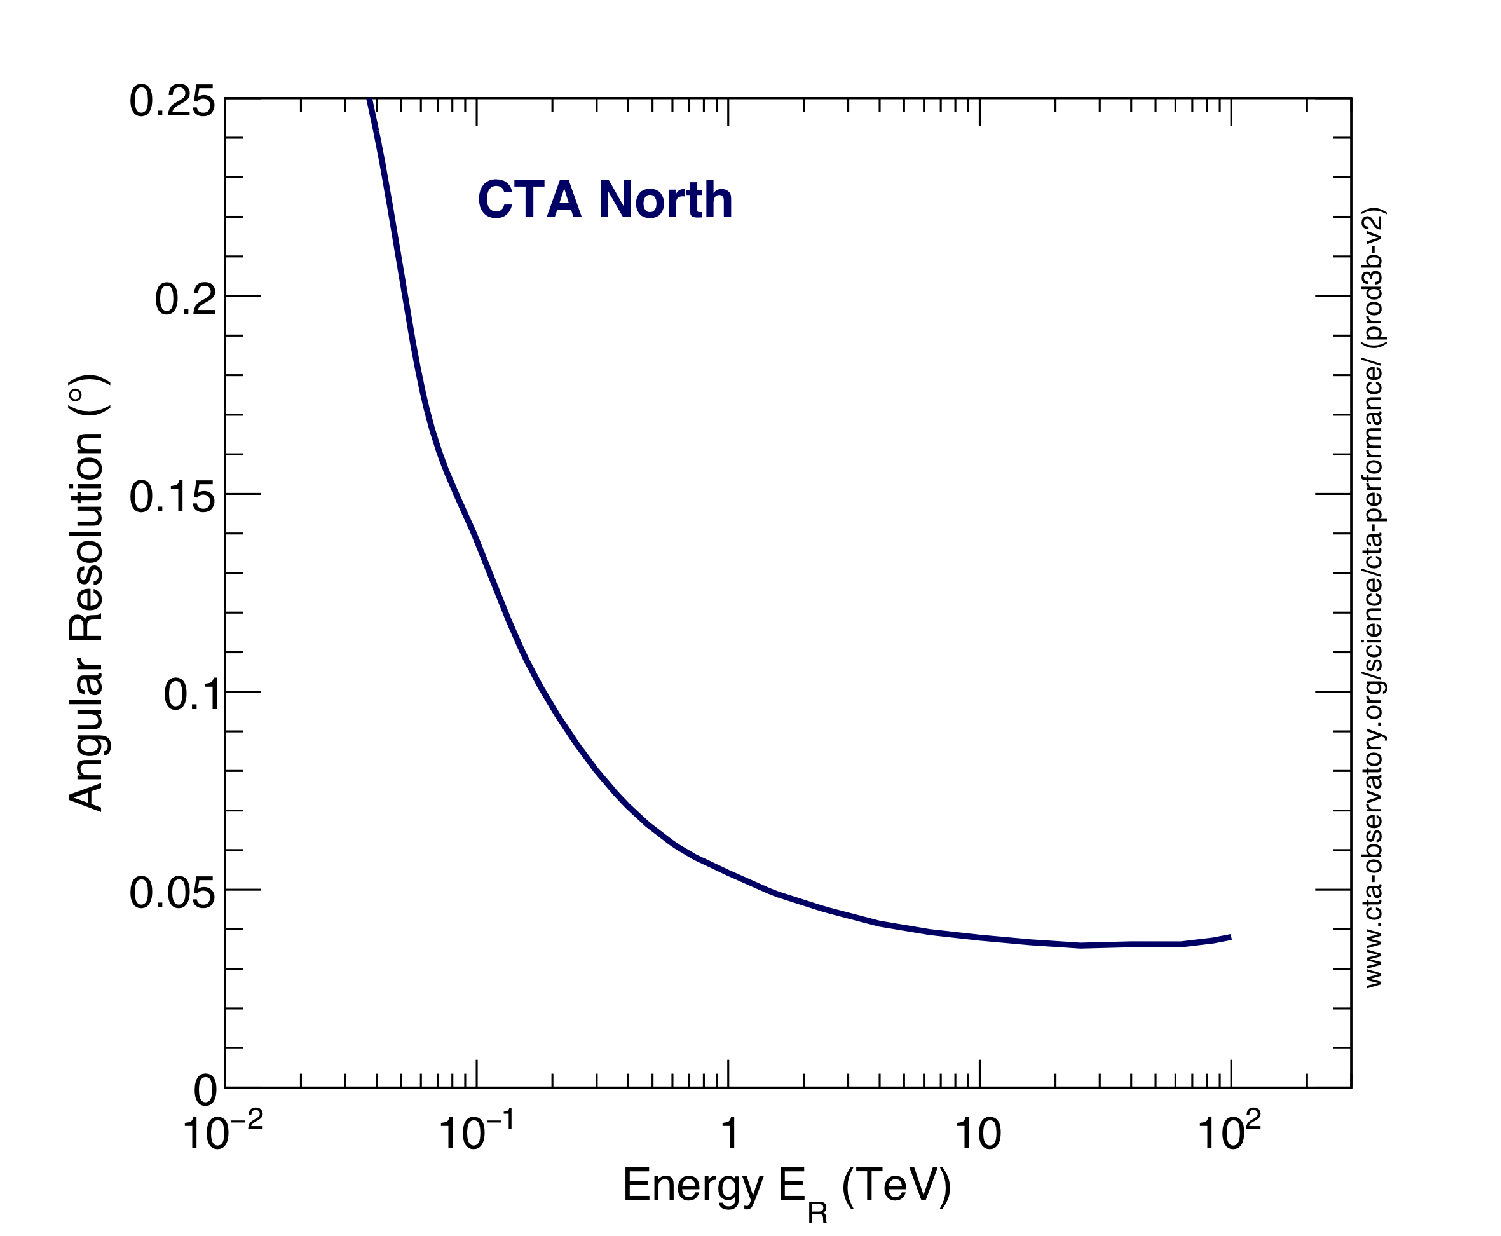
\includegraphics[width=\linewidth]{Pictures/CTA-Performance-prod3b-v2-North-20deg-AngularResolution.pdf}
    \endminipage\hfill
    \caption{\label{fig:angres} Angular resolution for CTA South compared to other experiments (left), and for CTA North (right) \cite{CTAPerformance}.}
  \end{figure}

\item \textbf{Energy resolution:} The energy resolution $\Delta E/E$ is obtained from the distribution $(E_{rec}-E_{true})/E_{true}$, where $E_{true}$ and $E_{rec}$ are the true and reconstructed energies of $\gamma$-ray events. It is defined as the half-width of the interval around 0 which contains the 68\% of the distribution. The energy resolution of \gls{cta} as a function of reconstructed energy is shown in figure \ref{fig:energyres}. Note that for the range of 1-10 TeV the energy resolution is well below the required 10\%.\\
    
  \begin{figure}[!htb]
    \minipage{0.5\textwidth}
    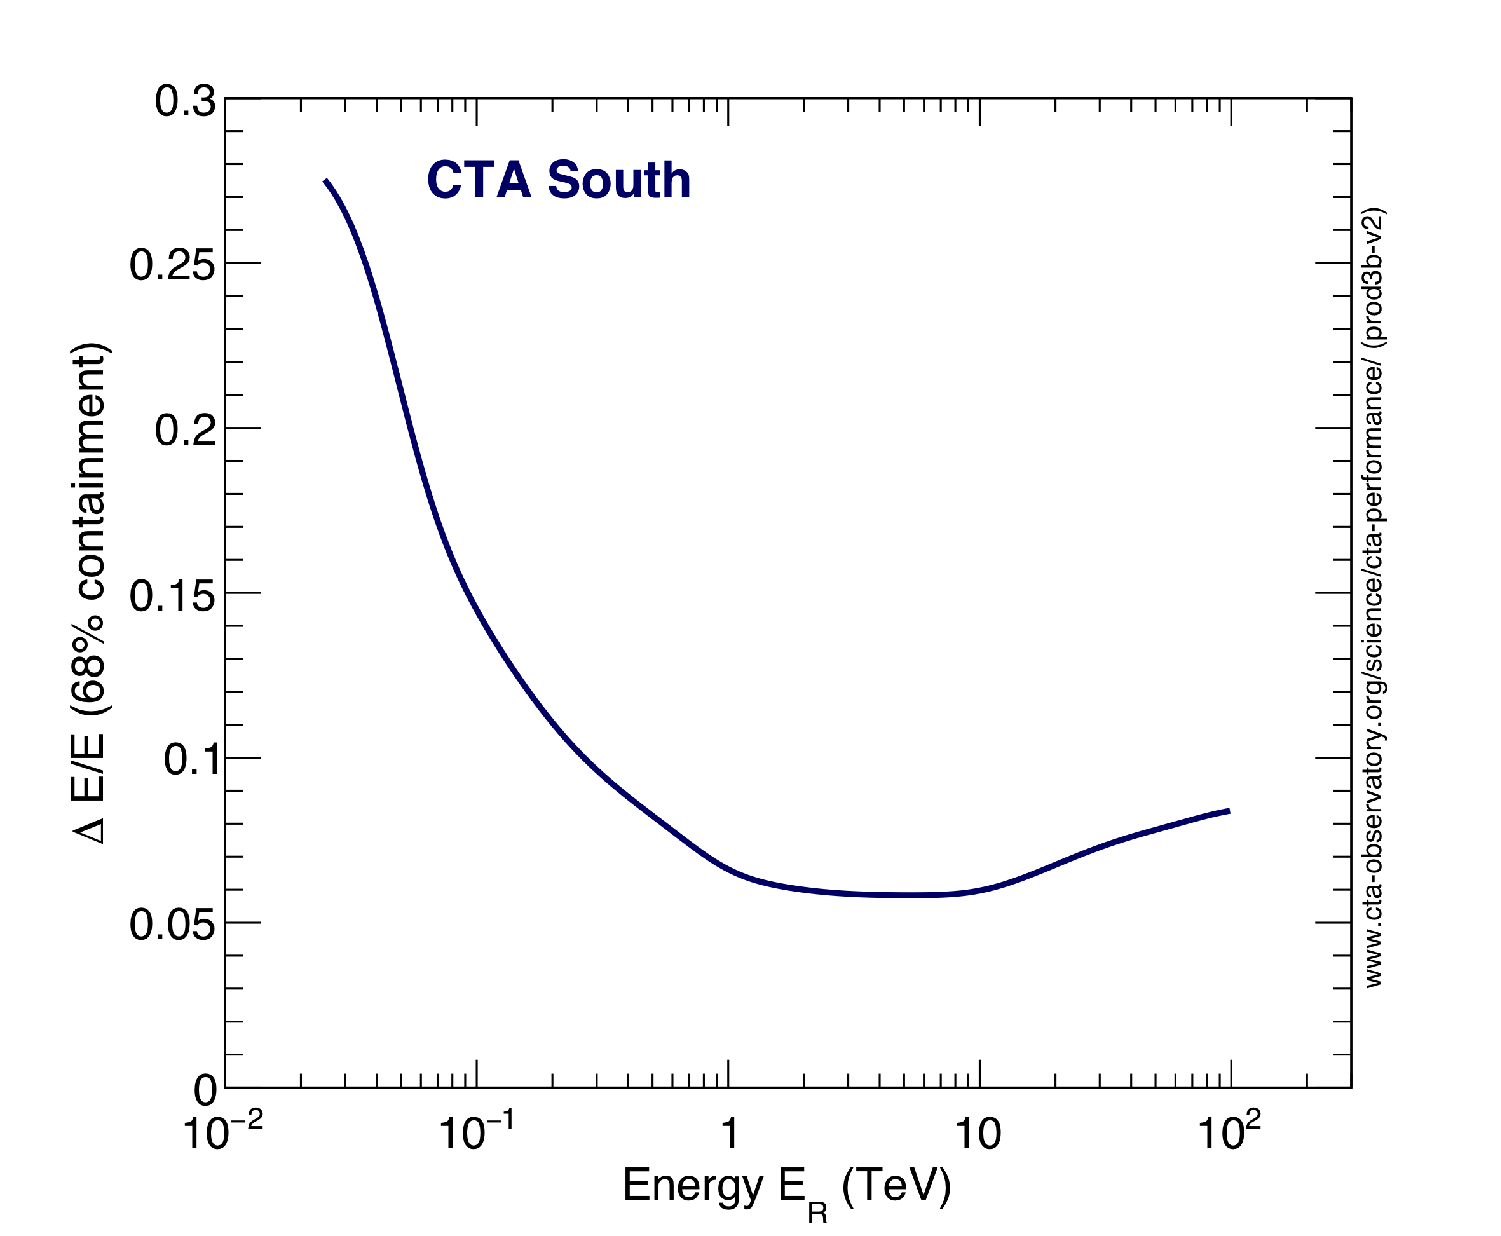
\includegraphics[width=\linewidth]{Pictures/CTA-Performance-prod3b-v2-South-20deg-EnergyResolution.pdf}
    \endminipage\hfill
    \minipage{0.5\textwidth}
    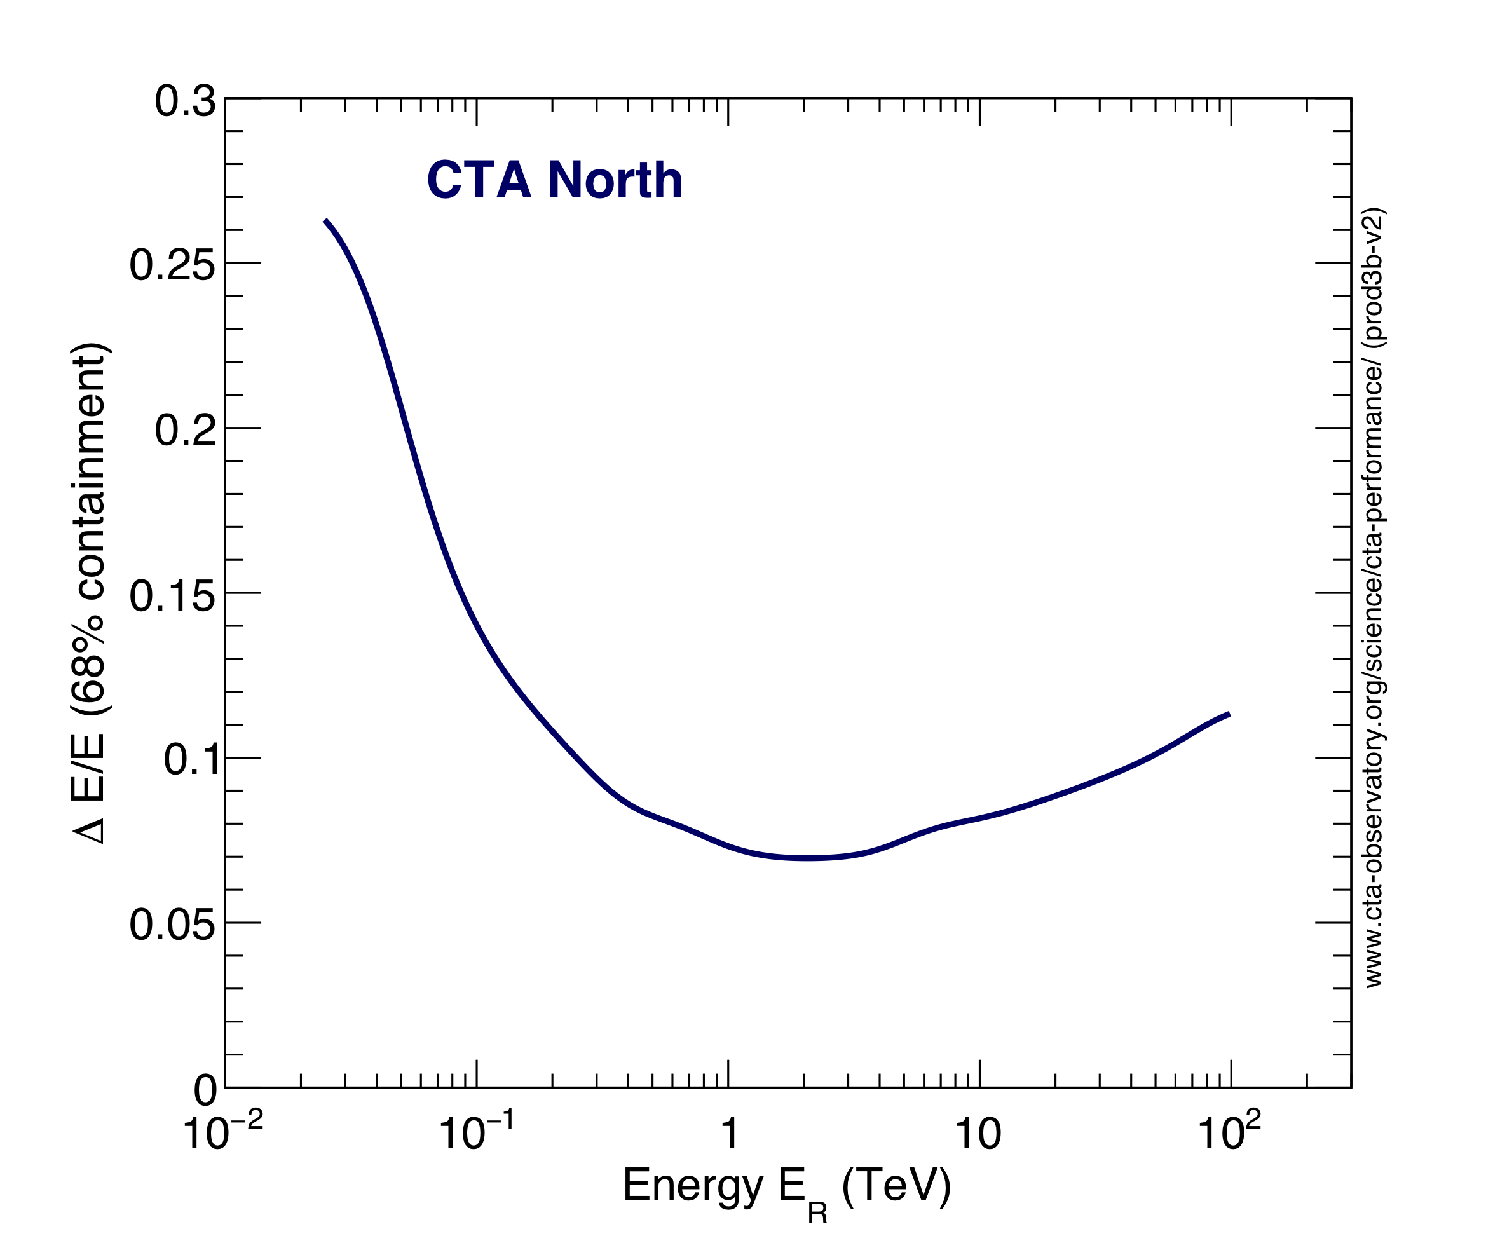
\includegraphics[width=\linewidth]{Pictures/CTA-Performance-prod3b-v2-North-20deg-EnergyResolution.pdf}
    \endminipage\hfill
    \caption{\label{fig:energyres} Energy resolution vs reconstructed energy for CTA South (left) and CTA North (right) \cite{CTAPerformance}.}
  \end{figure}
  
\item \textbf{Differential sensitivity:} The most important feature at evaluating the performance is the differential sensitivity, which indicates the minimum flux needed by \gls{cta} to detect a point-like source at $5\sigma$ in 50 hours. The sensitivity is calculated in five energy bins per decade, where it is required that at least 10 $\gamma$-rays are detected and the signal to background ratio is al least 1/20. The cuts in gammaness and source direction ($\theta^2$) are optimized to improve this quantity. The differential sensitivity of \gls{cta} compared to that of other instruments for 50h observation time is shown in figure \ref{fig:ctaperformance}.\\

\begin{figure}
    \centering
    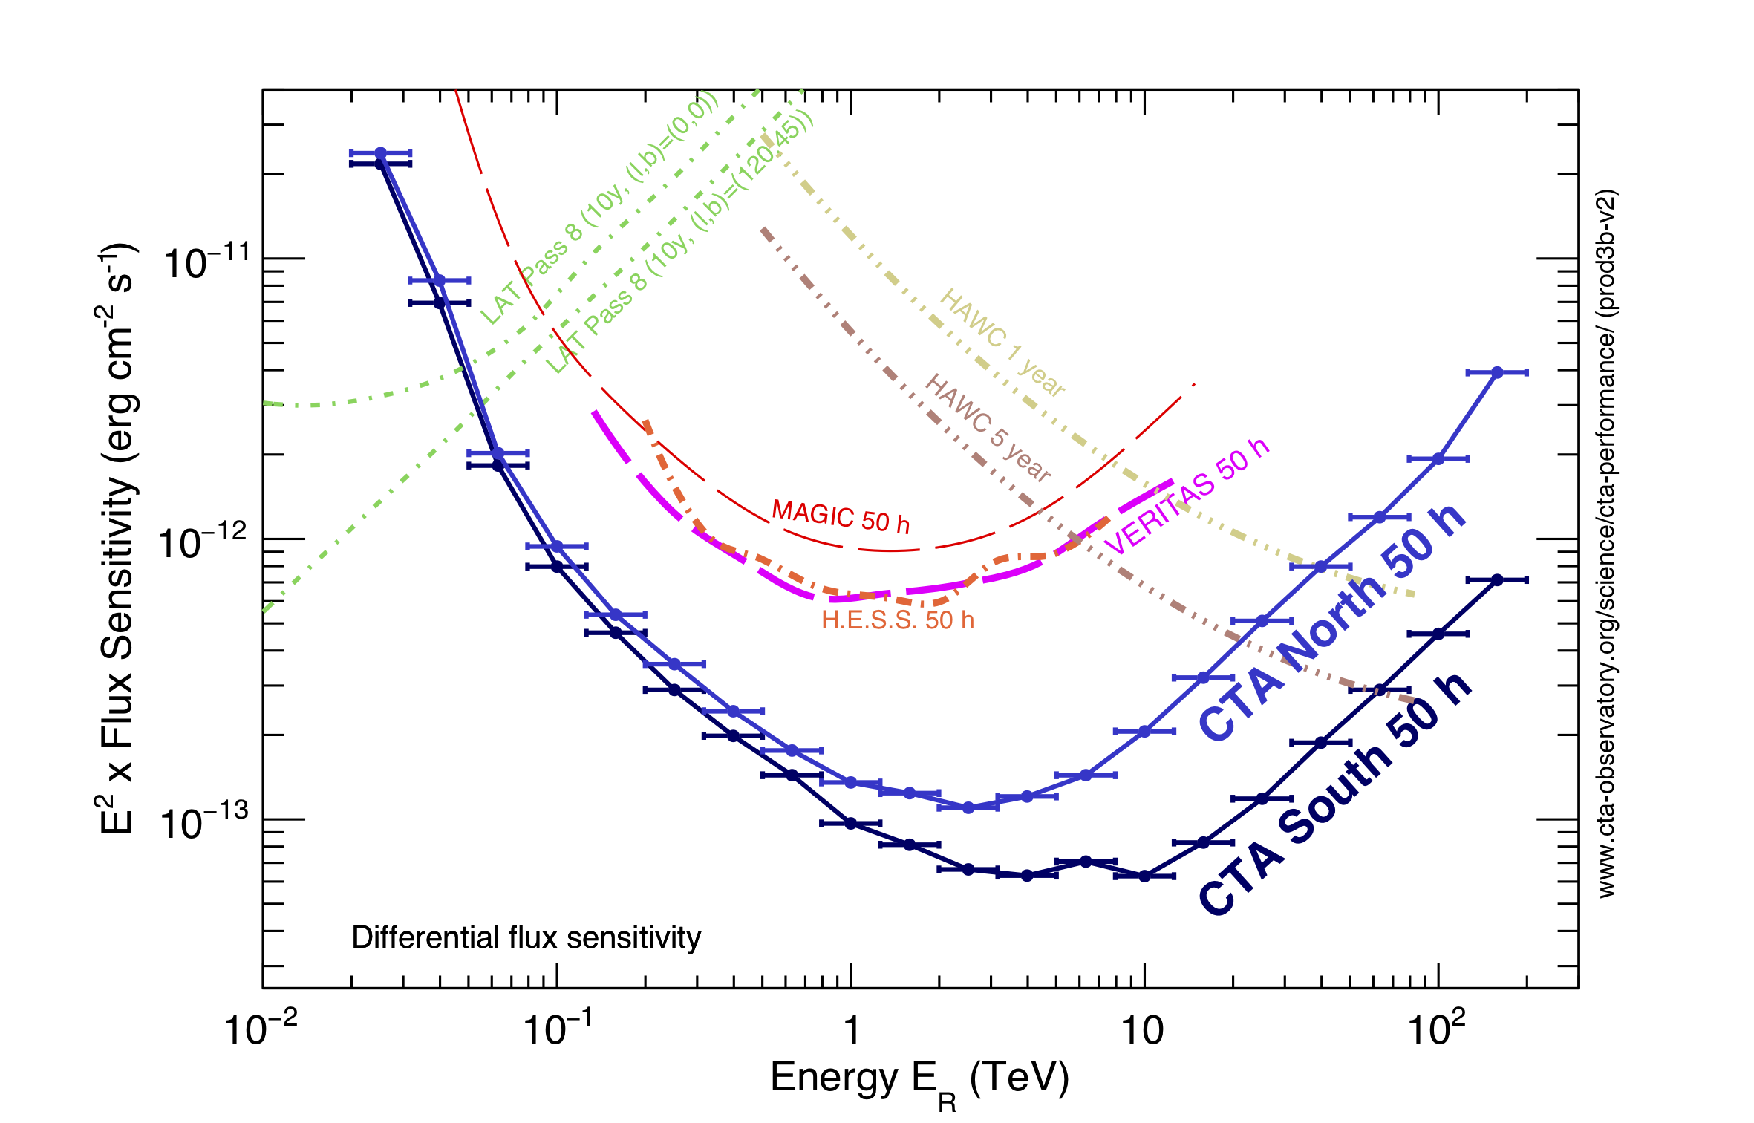
\includegraphics[width=1\textwidth]{Pictures/CTA-Performance-prod3b-v2-Comparison-DifferentialSensitivity-OtherInstruments.pdf}
    \caption{Differential sensitivity of \gls{cta} for 50 h observation compared to other $\gamma$-ray experiments, from \cite{CTAPerformance}.}
    \label{fig:ctaperformance}
\end{figure}
  
\end{itemize}

\section{CTA Telescopes} \label{sec:ctatelescopes}

While all telescopes share a basic design concept, they have particular features to accomplish the performance requirements for \gls{cta}. In general, subsystems of \glspl{iact} are divided in \textbf{structure}, \textbf{optics} and \textbf{camera}. 
In this section an overview of these subsystems and the particularities of each of the three types of \gls{cta} telescopes is given. 

\subsection{Large Size Telescope (LST)}

The \gls{lst} has been designed to reach an effective energy threshold down to20-30 GeV. This energy range has a particular interest because it covers the barely explored gap between the highest energies detected by satellite experiments, and the lowest by \glspl{iact}. The main science goals for \glspl{lst} are to observe high redshift \gls{agn}, \glspl{grb}, pulsars and galactic transients. The first prototype for the \glspl{lst} (\gls{lst}1) was installed in the CTA North site, in La Palma island, in 2018.\\
A detailed description of \gls{lst} subsystems can be found in \cite{2013LST}, next sections offer a summary of each subsystem of the telescope, which consists of: the structure of the telescope, to support the optics, camera and driving system; the optics, composed by the 23 m diameter mirror which collects the Cherenkov light and focus it in the camera; and the camera, to record the photons coming from the showers.  

\subsubsection{\gls{lst} Structure}

The structure of the telescope is divided in several parts: The azimuth system, the mirror support dish, the elevation system, the camera support structure and the drive system. All parts of the structure are specially designed to make the telescope lightweight ($\sim$ 100 tons), to ensure fast repositioning in the case of a transient alert (mainly \glspl{grb}), being able to re-position to any part of the sky within 20 seconds.\\
The azimuth system allows the telescope to turn around its vertical axis. It consists in a circular rail of 24 m diameter where six wheeled bogies support the structure. The azimuth structure is a framed structure made of \gls{cfrp} and aluminum tubes. The mirror support dish is a double layer space frame made of \gls{cfrp} tubes arranged in a tetrahedral structure, with a diameter of 23 m. The elevation system consists of a structure made in part of steel tubes, located in the backside of the dish, to help compensate the weight of the telescope and ensure the stiffnessof the structure. The camera support structure, which holds the camera frame, consists on an arch with three curve sections on each arm, made of \gls{cfrp}, and a total of 26 ropes to stiffen the structure. The drive system, designed to ensure a fast and precise repositioning, consist on 4 synchronous motors capable to supply a total mechanical power of 190 Kw to move the structure in azimuthal axis and elevation. The different parts of the structure are shown in figure \ref{fig:LST}.
    
  \begin{figure}[!htb]
    \minipage{0.5\textwidth}
    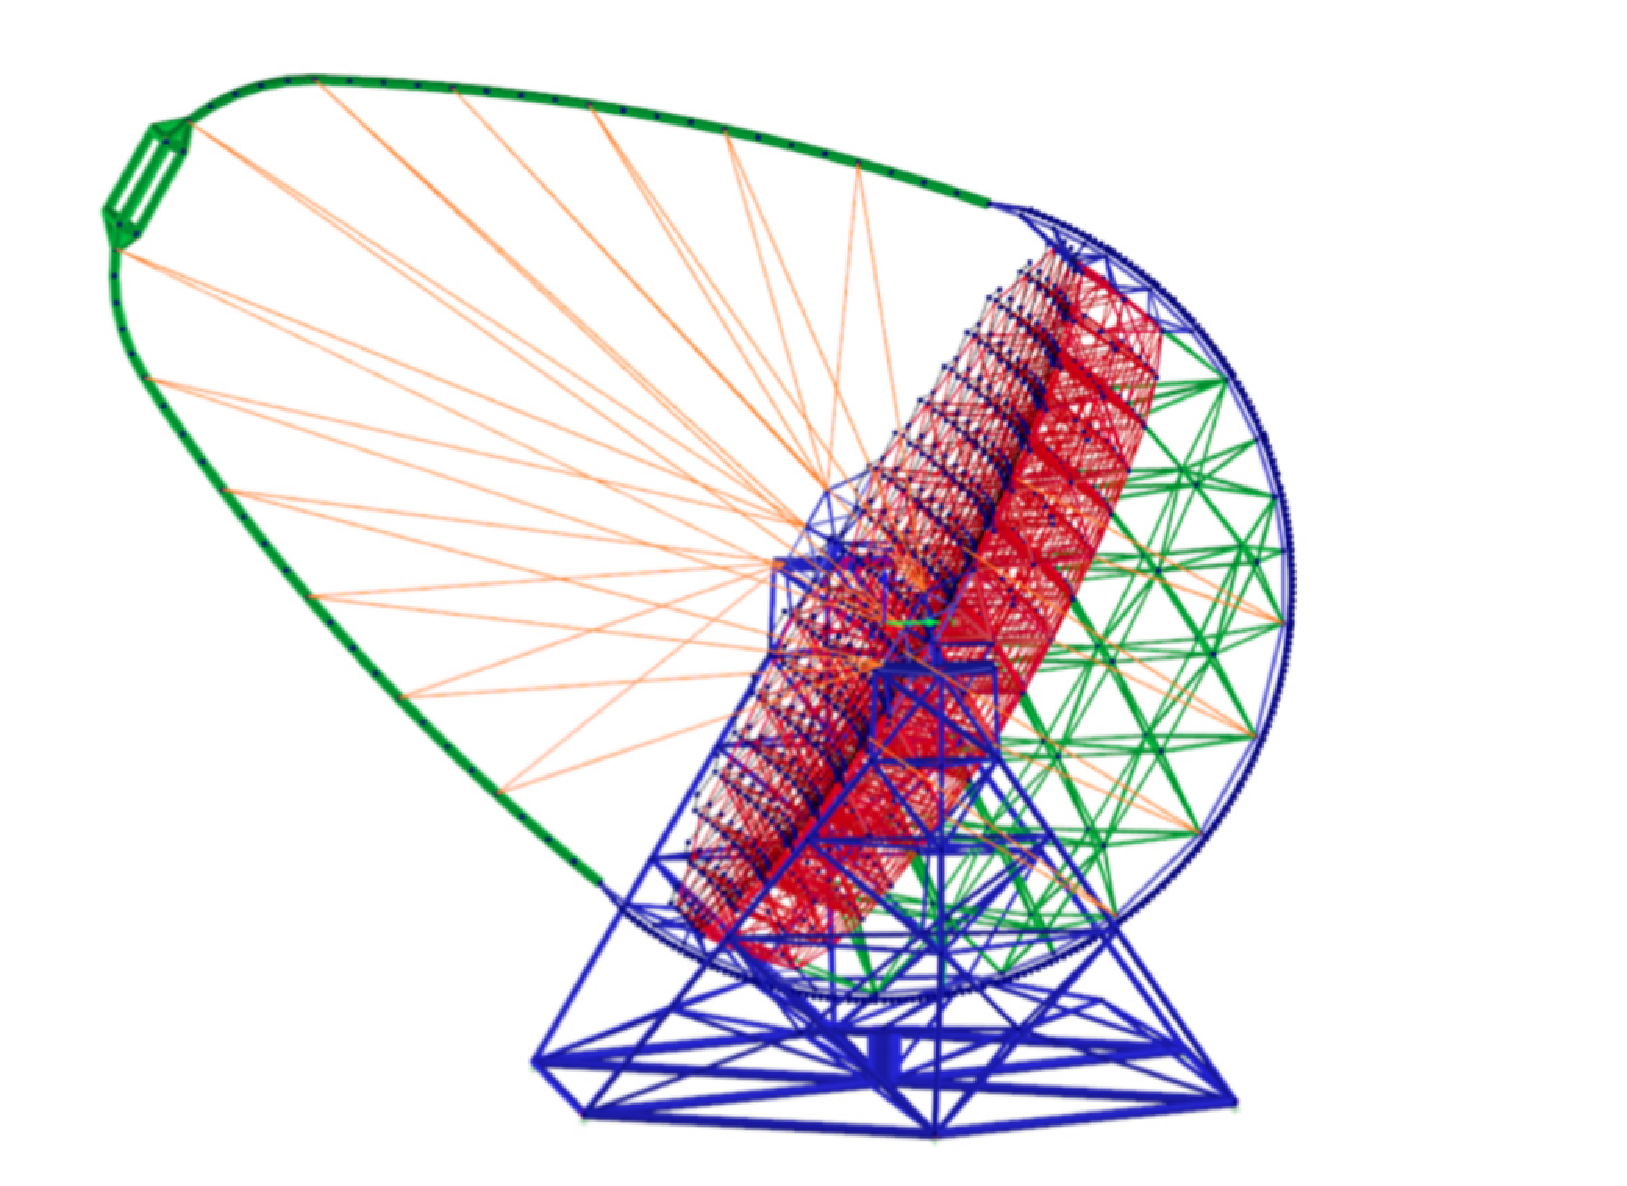
\includegraphics[width=\linewidth]{Pictures/LSTstructure.pdf}
    \endminipage\hfill
    \minipage{0.5\textwidth}
    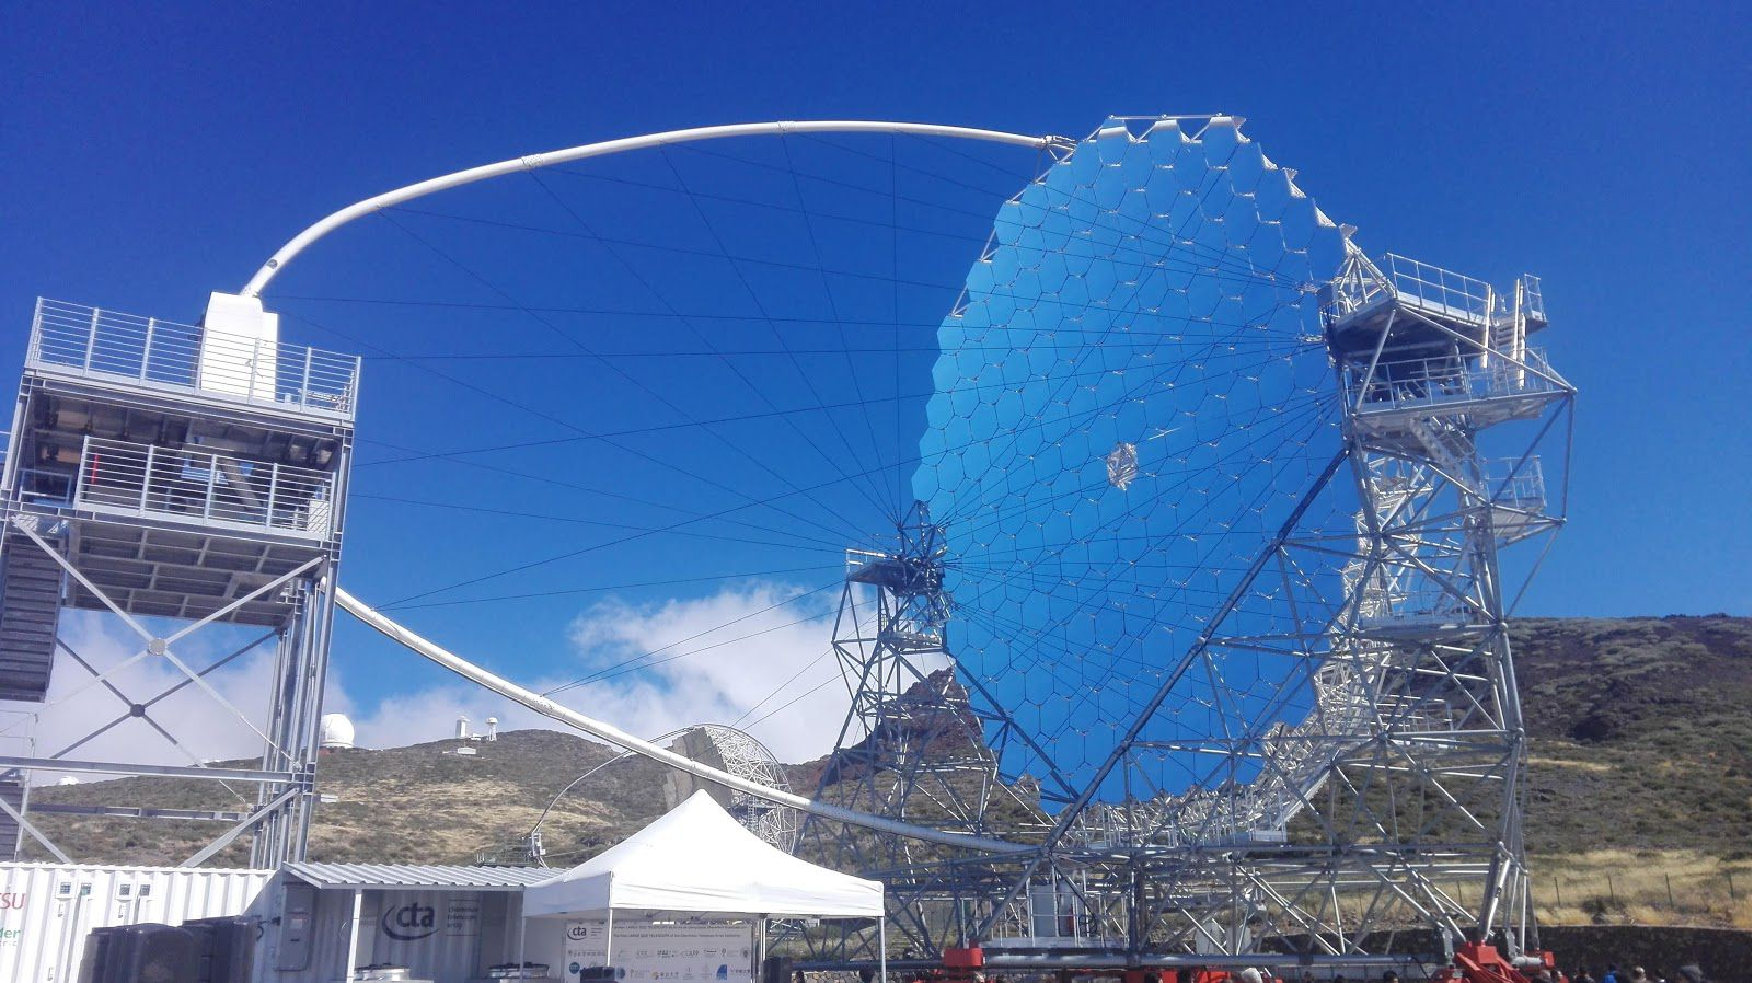
\includegraphics[width=\linewidth]{Pictures/LST1.pdf}
    \endminipage\hfill
    \caption{\label{fig:LST} Left: Simplified diagram of the structures of \gls{lst} without bogies, mirrors and camera. Azimuth substructure is blue color, the elevation system and the camera support structure are shown in green color and the mirror dish is red color, from \cite{2013LST}. Right: Photo of the first LST installed in CTA North site (Roque de los Muchachos Observatory, La Palma, Spain).}
  \end{figure}
  
  \subsubsection{\gls{lst} Optics}

  The mirror of the telescope has a parabolic shape, to guarantee the isochronousity of the optics. It has 23 m diameter, 28 m focal length and it is segmented in 198 hexagonal facets. The mirrors are manufactured using the cold slump technique consisting in producing a sandwich of an aluminum honeycomb structure between two glass sheets \cite{2017LST}.
Mirrors are fixed to the telescope structure by three knots, two of them mounted on actuators which allow to adjust each mirror panel in two directions. The \textit{active mirror control} system controls these actuators in order to fine tune the focal distance and focusing, to account for the possible deformations and bending of the telescope structure. Each mirror segment is equipped with an infrared laser, and two more lasers are mounted in the center of the disk, which constantly point to the left and right of the camera. The directional offset of the mirror facets can be estimated by taking pictures of the reflected spots on a target in front of the camera with a high resolution IR CCD camera located in the center of the dish. The achievable positioning resolution can reach $< 5 \mu m$ \cite{2013LST}.
  
  \subsubsection{\gls{lst} Camera}

  The camera focal plane instrumentation consists of 256 modules (sometimes also referred as clusters) with seven \glspl{pmt} each, making a total of 1855 pixels. The \glspl{pmt} are mounted with a 50mm pitch, coupled to hexagonal light guides made of a reflective material (3M ESR), to collect all the light arriving to the camera. The \gls{pmt} model is Hamamatsu R11920-100-20, specially developed to reach high quantum efficiency (42\%) and low after pulse rates, which go below 0.02 \% above 4 photoelectrons. Each module with seven photodetectors has one readout system based on the \gls{dsr4}. The signal from the \glspl{pmt} is split in three branches: high and low gain ones, which are sampled at $\mathcal{O}$(GS/s) in the \gls{dsr4} chips; and the trigger branch, which is feed into the Level 0 trigger asic \cite{2017LST}. A slow control board monitors the \glspl{pmt} and controls the high voltage elevators. Analogue backplanes are dedicated to trigger distribution along modules and clock signal propagation.  
  The mechanical structure of the camera consists of several parts, shown in figure \ref{fig:LSTcammech}. The modules are inserted in the load bearing structure from the front of the camera and connected to the backplane electronics on its rear part. The design of such modular structure guarantee an easy access to individual modules in case any repair is necessary, allowing to disconnect and extract one module without manipulating the rest of the camera.
  The load bearing structure is mounted inside the tubular structure which holds the camera external walls, doors and interfaces with the camera frame. In the front part of the camera there is the front window which can be totally covered by a shutter to avoid the entrance of sunlight during the day to maximize the life of the \glspl{pmt}. In the back part of the camera lies all the cabling and auxiliary electronics. The total dimensions of the camera is $2.9\times2.9\times 1$ m$^3$ and the weight is less than 2000 kg. Since all the electronics are stored inside the camera, the structure was required to accomplish a series of requirements related to the exposure to environmental conditions such as the protection to the entrance of dust, water and sunlight and guarantee a stable temperature between 20ºC and 40ºC \cite{2013LSTCamMech}. Temperature regulation is possible thanks to the water cooling system, based on cold plates and a temperature controlled air flow cooling system.\\
 An access tower allows to intervene in the camera during day-time operations when the telescope rests in park position, and also acts as an anchor in case of strong winds. 

\begin{figure}
\centering
 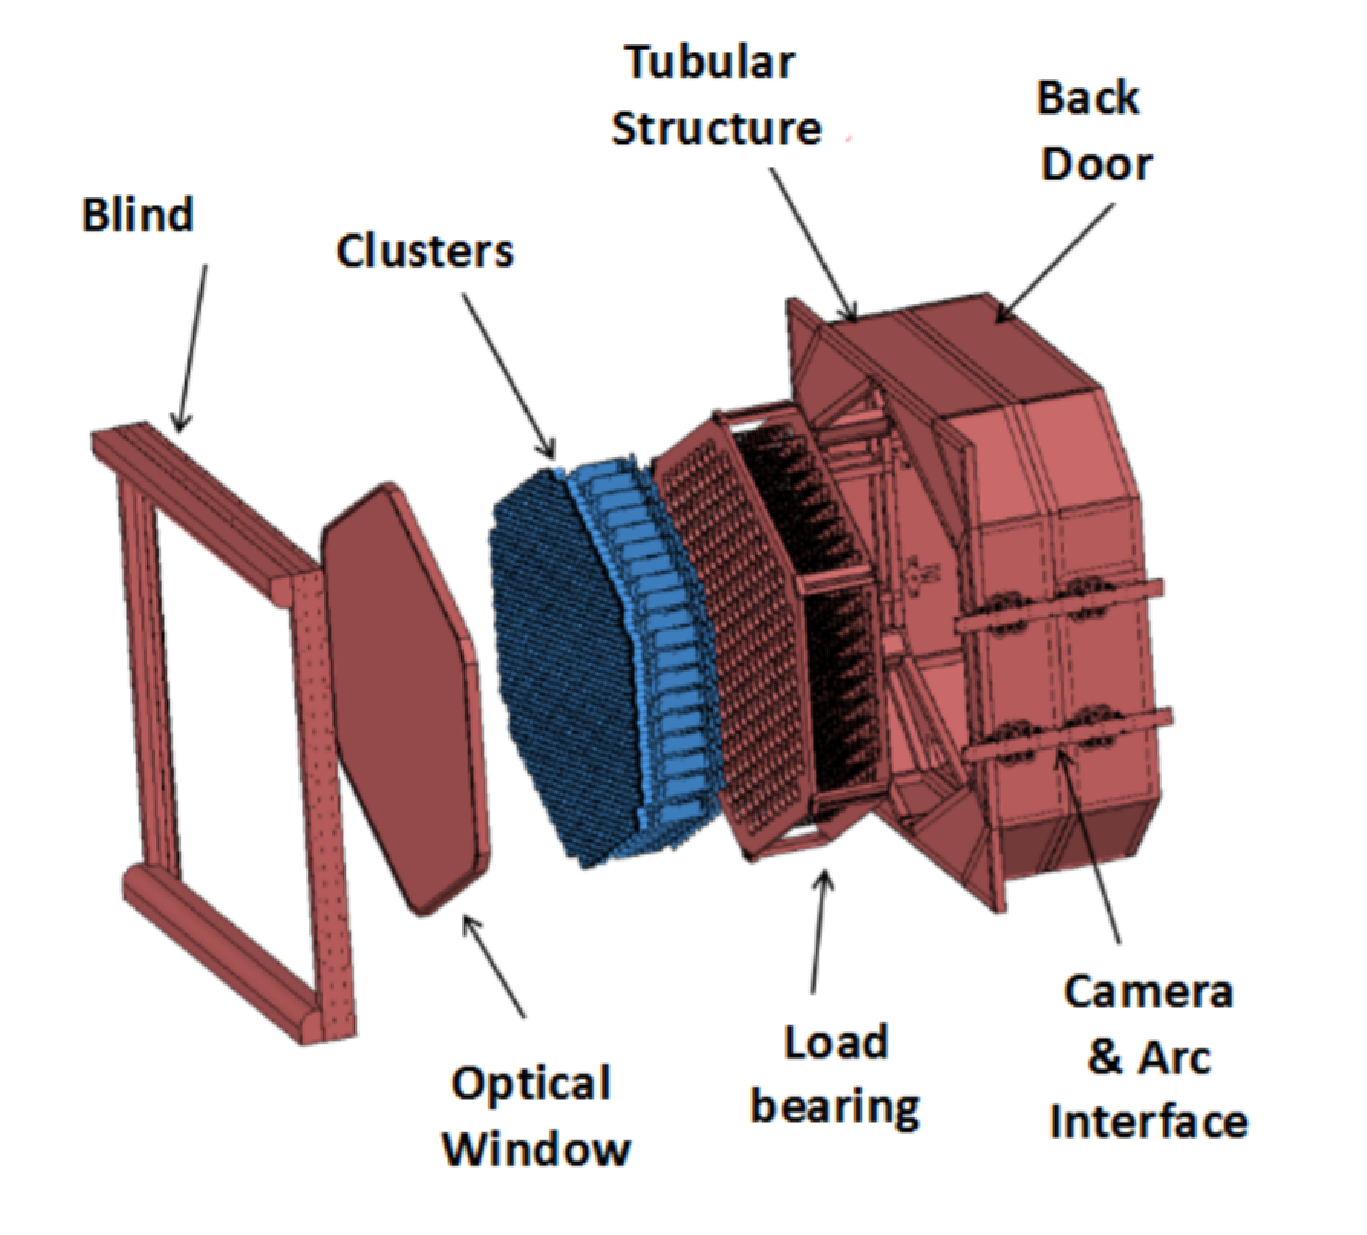
\includegraphics[width=0.7\textwidth]{Pictures/LSTcamerastructure.pdf}
  \caption{Different \gls{lst} camera mechanical elements from \cite{2013LSTCamMech}.}
    \label{fig:LSTcammech}
\end{figure}

\subsection{Medium Size Telescope (MST)} \label{sec:MST}

\glspl{mst} will cover the core energy range of \gls{cta}, from 100 GeV to $\sim 10$TeV. This is the usual range reached by current \gls{iact} generation so the improvements in sensitivity will come from the large area covered and the better image reconstruction due to the larger number of telescopes (15 in the north, 25 in the south).
The \gls{mst} 12 m diameter modified \gls{dc} optical layout very similar to that of \gls{veritas} and \gls{hess}. The first prototype of this type, the \gls{dcmst} \cite{2017SCMSTstatus}, was built in Adlershof, Germany. There are two different camera designs for \gls{dcmst}: \textit{FlashCam} and \textit{NectarCAM}, which characteristics will be discussed in this section.
A detailed report of the status of the \glspl{mst} as of July 2019 can be found in \cite{2019MSTreport}. A summary on the different parts of the telescopes is given in this section.

\subsubsection{\gls{mst} Structure}

The structure of the \gls{mst} can be seen in figure \ref{fig:2MST}.
The main mechanical structure of the telescope is a cylindrical tower of 1.8 m diameter and 20 mm wall thickness. The tower is connected on top to the head of the telescope, that contains the azimuth bearing which allows the telescope to rotate in the horizontal axis, and the drive assemblies. It is possible to access to the tower through a door at the base. All electrical cabinets are stored and distributed over three floors of the tower. A combination of ventilation and air conditioning system is used to keep the temperature within the cabinets operation range.
The drive assemblies are designed to reach any object above 30º in elevation in less than 90s. It is divided in the azimuth drive subassembly and two elevation drive subassemblies, mounted in the left and right of the telescope.
To account for the possible sources of excitation, like wind gusts or structure flexibility, which can lead to oscillations of the structure, an active vibration damping control is used to reduce their effect on the pointing accuracy of the telescope.
The dish structure is designed to host the mirrors and the camera support structure is attached to it \cite{2015DCMSTstatus}.

\begin{figure}
\centering
 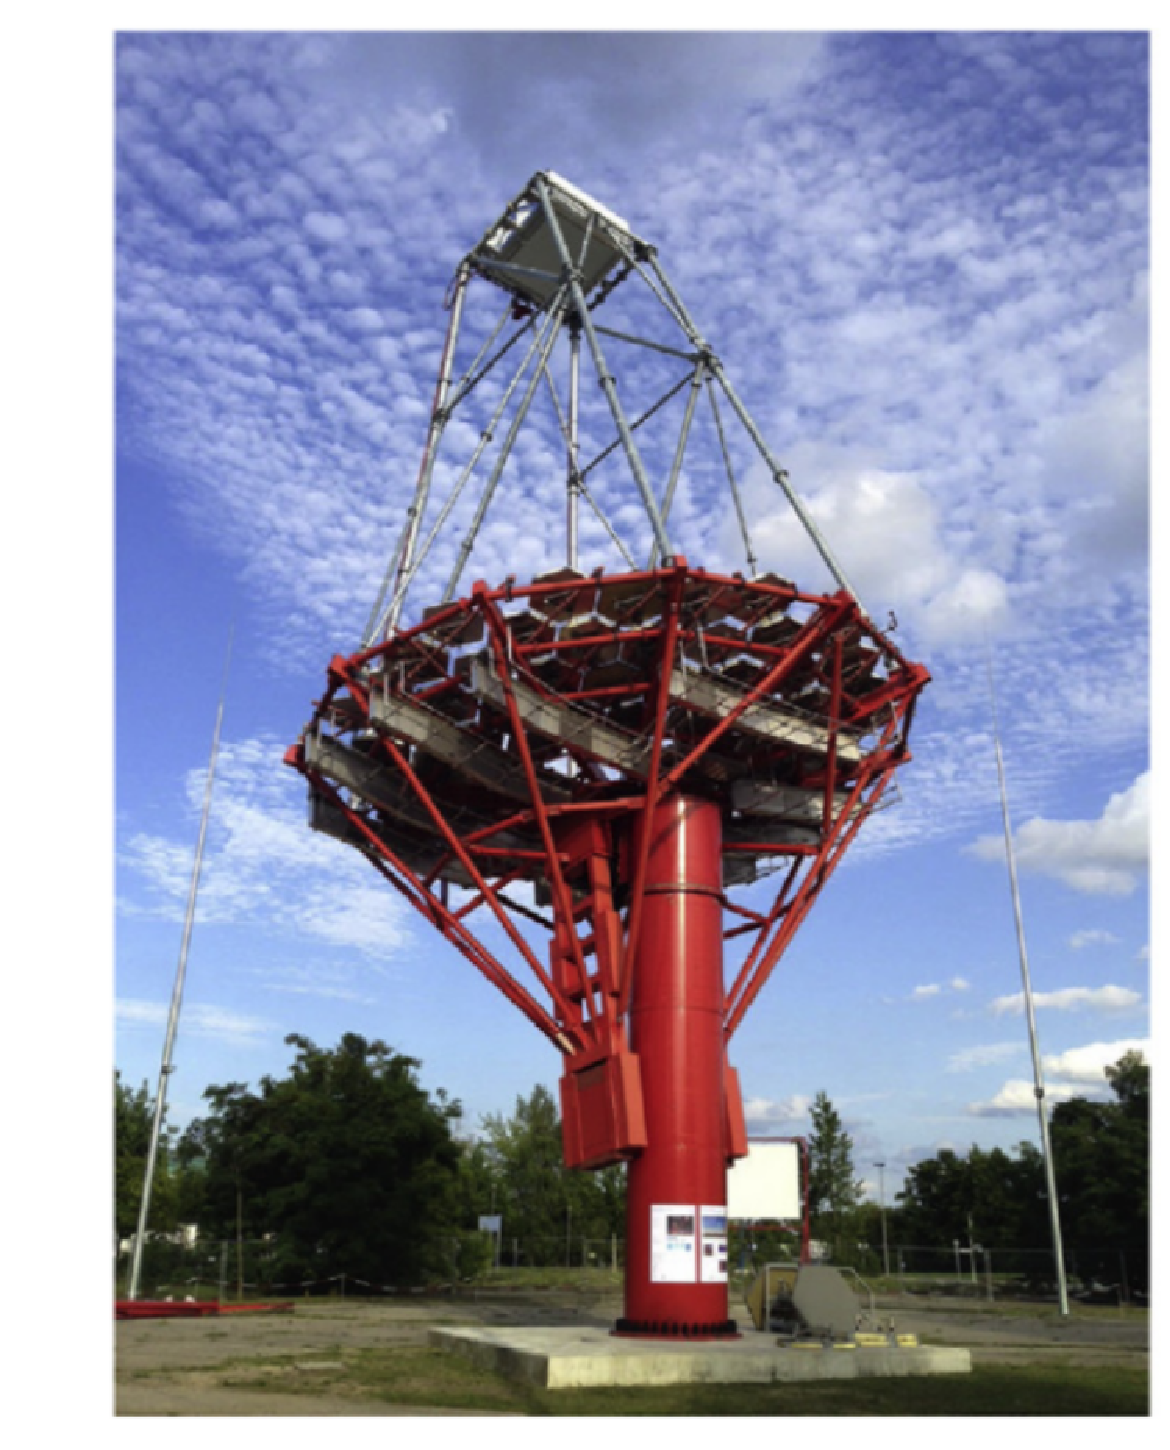
\includegraphics[width=0.7\textwidth]{Pictures/MST.pdf}
  \caption{\gls{dcmst} prototype with FlashCam in Adlershof, from \cite{2018MSTandLSTstatus}.}
    \label{fig:2MST}
\end{figure}

\subsubsection{\gls{mst} Optics}

The optical system of the \gls{dcmst} consists on a mirror segmented in 86 hexagonal facets of 1.2m length, providing an effective mirror area > 88 m$^2$. The focal length of the telescope is 16 m.
Different mirror technologies are being tested, all based in cold slumping technique, with different layers of materials, coatings and structures. A system of actuators forms the \gls{amc} system of the \gls{mst} allowing to adjust the mirror position for focusing. The structure is stiff enough to make unnecessary to readjust during observations to maintain the \gls{psf}. The \gls{amc} is used only for the initial mirror adjustment and for maintenance activities, or adjust the focal distance for specific observations.

\subsubsection{\gls{mst} Cameras}

Two camera prototypes have been designed and tested in the structure installed in Adlershof and showers have been detected, as shown in picture \ref{fig:MSTcamerasimg}.
The first design named FlashCam have 1764 \gls{pmt}-based pixels divided in 147 modules of 12 pixels each. It implements a fully-digital trigger and readout system operating at 250 MS/s which allows to define flexible trigger patterns relying on the digitized \gls{pmt} signals. The readout system is designed for a dead-time-free operation with trigger rates up to 30 kHz. FlashCam uses only one gain channel, reducing the required bandwidth for data transfer. 
The second camera design named NectarCAM counts with 1855 pixels, divided in 256 groups of 7 modules. The camera mechanics and many auxiliary systems have been designed to be equivalent to the \gls{lst} camera. The signal digitizing of NecatrCAM relies on a dedicated Nectar ASIC which digitizes the \gls{pmt} signals at sampling speeds of around 1 GHz. It implements a digital trigger based on the binary outputs of individual pixels after comparing their analog signals with a threshold (Level 0 trigger).\\

\begin{figure}
\centering
 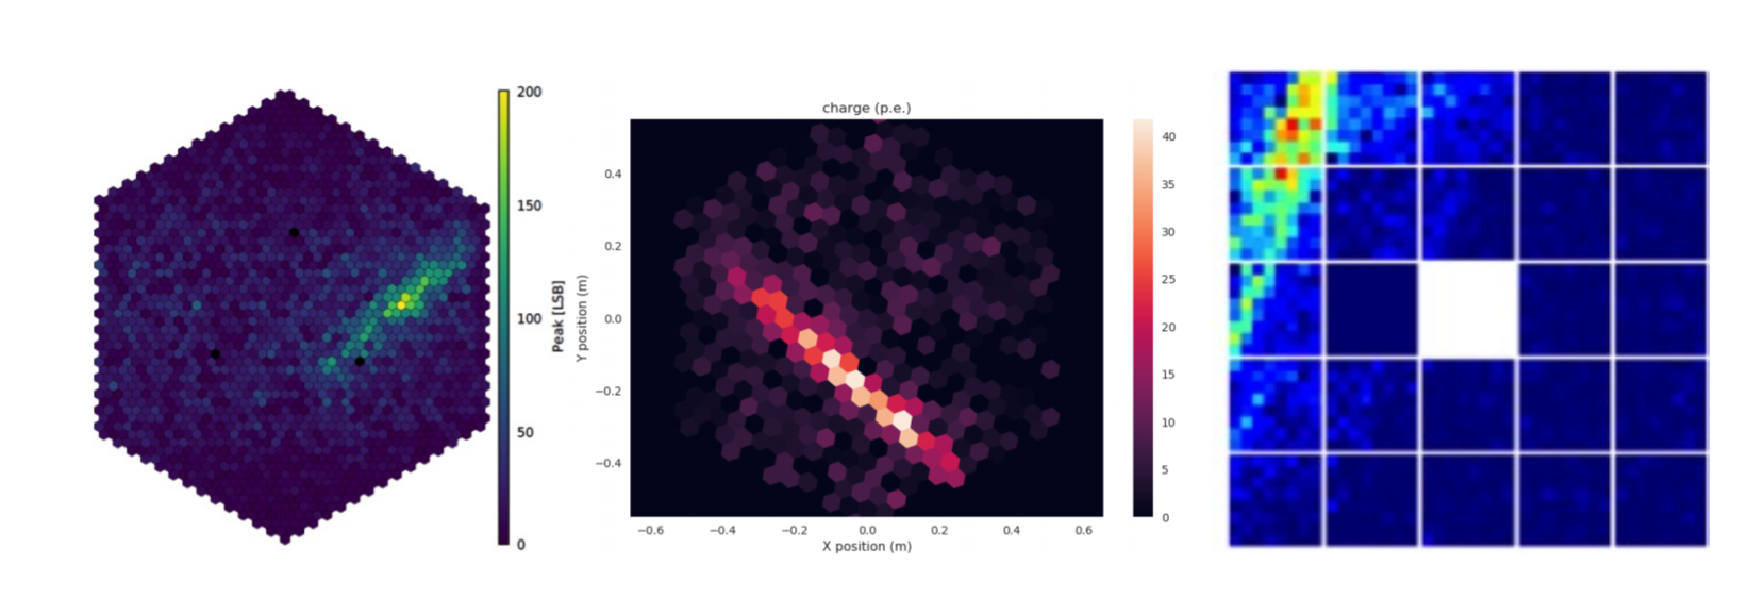
\includegraphics[width=\textwidth]{Pictures/showerimagesMST.pdf}
  \caption{Left: \gls{dcmst} Showers obtained with FlashCam(\textit{left}), NectarCAM(\textit{middle}) and \gls{scmst} camera (\textit{right}) prototypes, from \cite{2019MSTreport}.}
    \label{fig:MSTcamerasimg}
\end{figure}

\subsection{Small Size Telescope (SST)}

The smaller telescopes, \glspl{sst}, will be the more numerous in the \gls{cta} layout, with more than 70 telescopes in the southern site. These telescopes are dedicated to detect the highest energy $\gamma$-rays which in the majority of cases will come from the galactic plane. They need to be spread over a very large area, to catch as many $\gamma$-ray showers as possible, but they do not need large mirrors because \gls{vhe} radiation produces a huge amount of Cherenkov light. They are designed to reach their peak sensitivity at energies greater than 10 TeV.

\subsubsection{\gls{sst} Structure}

The optical design of \glspl{sst} is based on a \gls{sc} double mirror configuration. A column raises from the base of the telescope and interfaces at the top with the azimuth fork. The fork sustains the elevation assembly, which is composed by the mirror dish, the counterweight and the structure that sustains the two mirrors. The dish is designed to hold the segments of the primary mirrors, which can be individually controlled by actuators. A quadrupod is attached to the dish, which together with a central pole, are joint to the structure that supports the secondary mirror and also serves to counteract deformations due to gravity and wind. The structure for the monolithic secondary mirror accounts for three actuators and three lateral arms which support the transverse components of the mirror's weight. The drive of the azimuth is located at the base of the column. A scheme of the structure can be found in picture \ref{fig:SST}. A detailed description of the \gls{sst} structure design can be found in \cite{2013SSTstruct}.

    
\begin{figure}[!htb]
  \minipage{0.4\textwidth}
  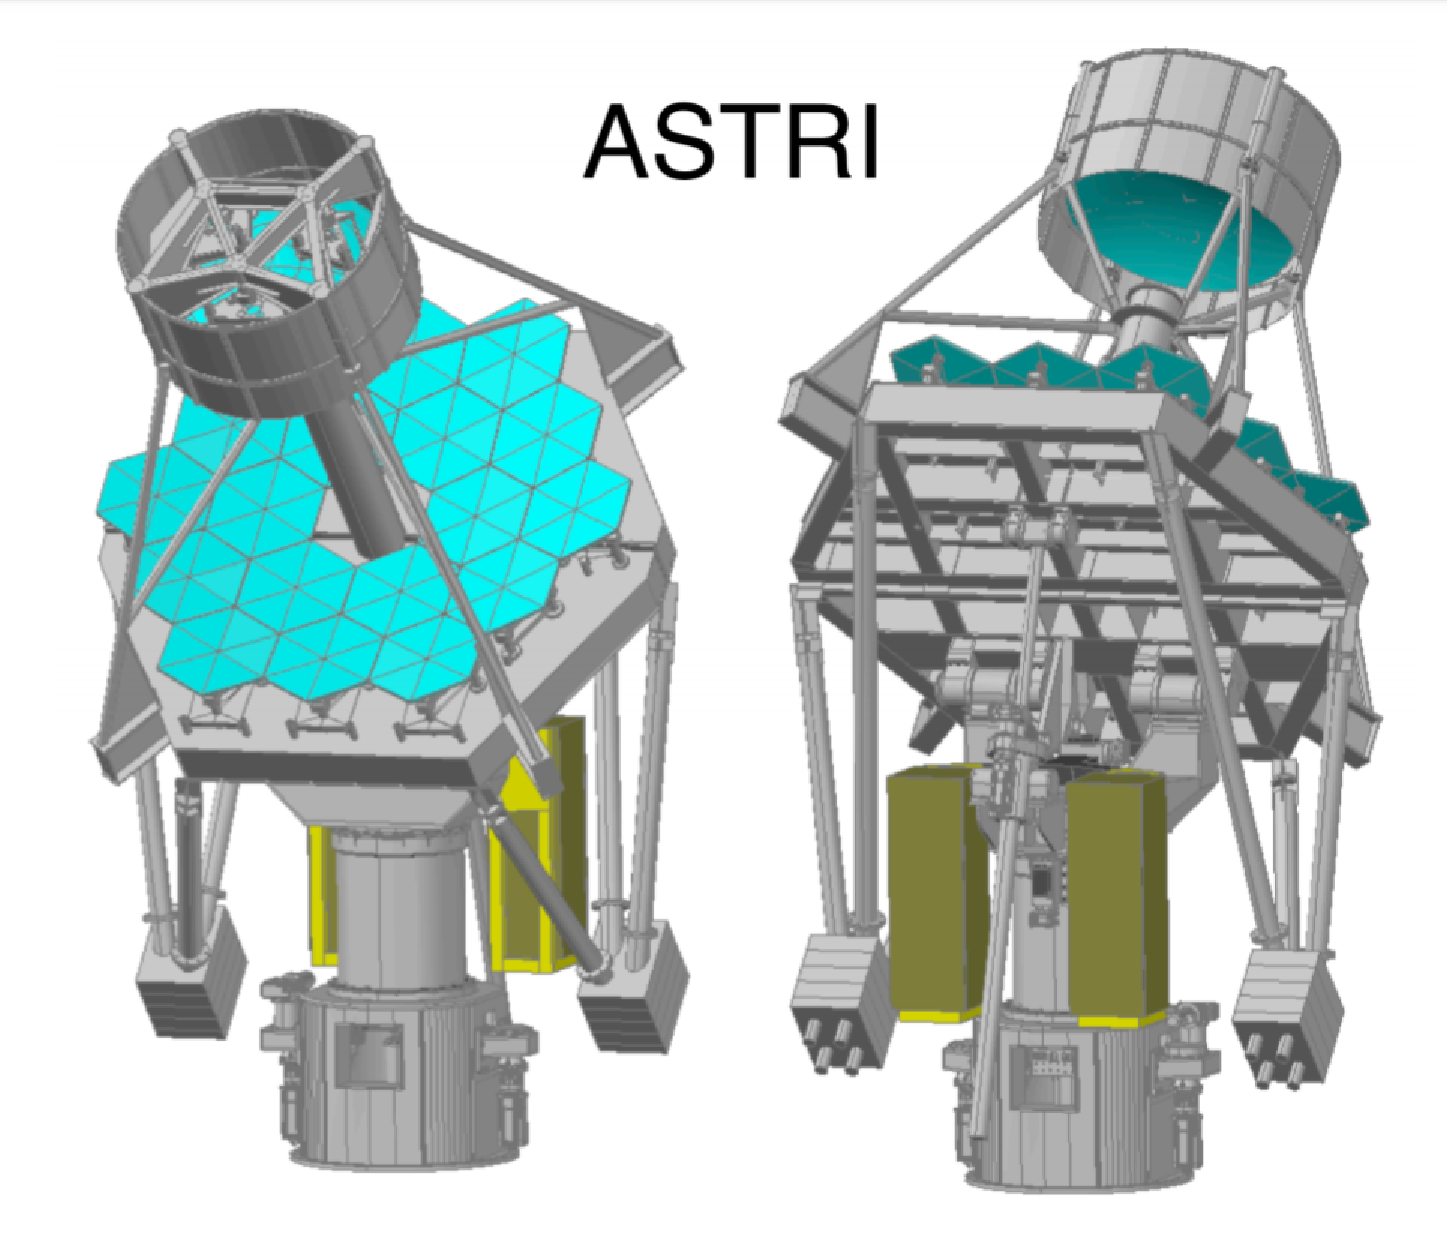
\includegraphics[width=\linewidth]{Pictures/ASTRI.pdf}
  \endminipage\hfill
  \minipage{0.6\textwidth}
  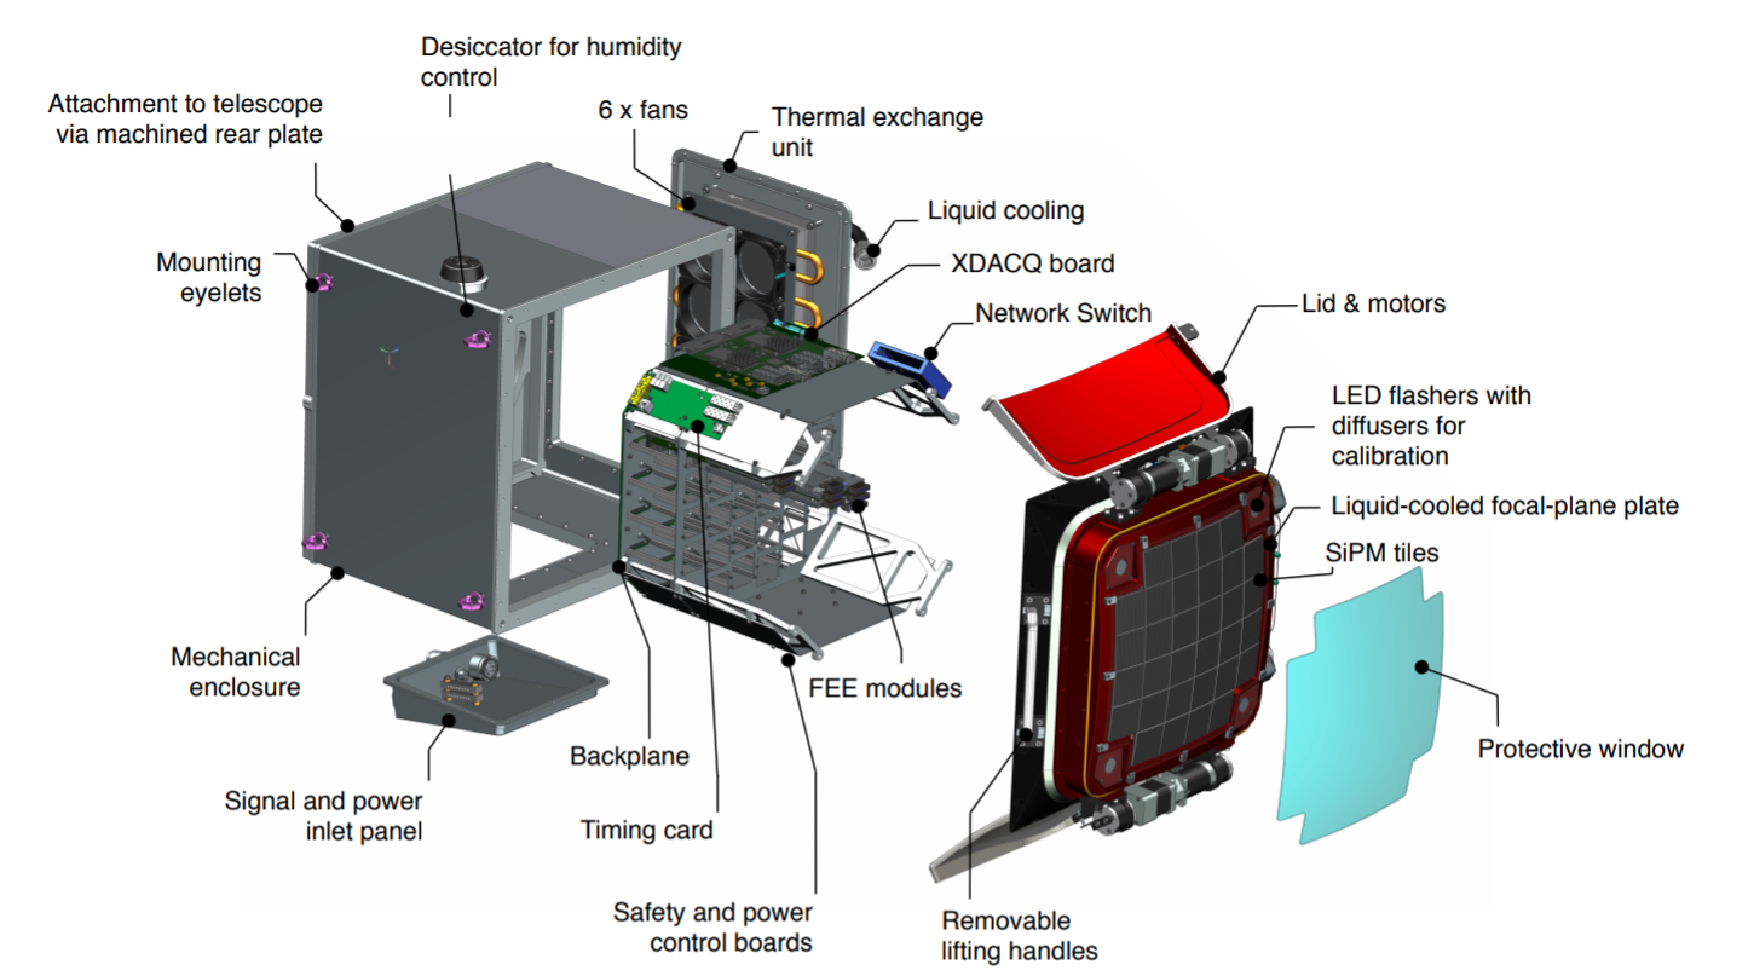
\includegraphics[width=\linewidth]{Pictures/CHECcam.pdf}
  \endminipage\hfill
  \caption{\label{fig:SST} \textit{Left}: General view of the \gls{sst} structure and electromechanical subsystems, adapted from \cite{2013SSTstruct}. \textit{Right}: CAD model of the \gls{chec} camera from \cite{2017CHECcam} }
\end{figure}

\subsubsection{\gls{sst} Optics}

The \gls{sc} design of the \glspl{sst} is composed by two mirrors, one primary of 4.3 m diameter segmented in hexagonal tiles, and a monolithic secondary mirror of 1.8 m. The primary mirror tiles have been manufactured using a cold slumping replication process. The secondary is made of a hemispherical thick glass shell thermally bent to 2.2 m radius of curvature. The focal length of the system is 2.15 m, f/0.5 and the \gls{fov} reaches 10º.\\
The advantages of a double mirror configuration are a better \gls{psf} over a large \gls{fov} and better correction of aberrations \cite{2017ASTRItels} than for single mirrors.

\subsubsection{\gls{sst} Camera}

The camera is composed by 2048 pixels made of \gls{sipm}, instrumented in 32 modules which comprise 64 pixels of $\sim 6\times6$ mm$^2$. The digitalization of the waveform is performed by \gls{fee} based on TARGET ASICs \cite{2017TARGETASIC} which also give the first trigger level, as the sum of four neighbouring pixels. A backplane provides the power, clock, trigger and data interface of the \gls{fee}. The trigger decision is formed in the backplane by combining trigger signals from all the \gls{fee} modules. In the camera structure, a lid protects the camera from the environment and a cooling system based on the circulation of chilled liquid through the camera focal plane plate and six internal fans, maintains a stable temperature. A diagram of the camera is shown in figure \ref{fig:SST}. A detailed description of the camera and results from its commissioning phase can be found in \cite{2017CHECcam}.

\section{Reconstruction and Analysis tools} \label{sec:ctaanalysis}

The best performance results from \gls{cta} with respect to the current generation \glspl{iact} will come not only from the telescopes designs, but it is also very important to have solid software tools, accessible and user friendly, which will allow to analyze the forthcoming data. Also, especially during the initial phases of the development of the facility, to calculate the predicted sensitivity shown in section \ref{sec:ctaperformance} it is necessary to produce precise and reliable simulations of the instrument response to the arrival of electromagnetic showers. In this section, the main software tools for the simulation and analysis of the different levels of \gls{cta} data are described. 

\subsection{Monte Carlo simulations}

\gls{mc} simulations are of great importance for the \gls{iact} technique, where the detection of $\gamma$-rays is indirect and it is necessary to reconstruct the primary parameters from the signal received at the telescopes. Detailed simulations of the development of the \gls{eas} in the atmosphere, combined with simulations of the instrument response to the Cherenkov light produced by those \gls{eas} are used for two main purposes: Separation of $\gamma$ and hadron showers and reconstruction of the shower direction and energy of the primary. For the former, since hadrons produce the majority of Cherenkov light which reach \glspl{iact}, it is necessary to characterize the particular differences between photon and hadron induced showers thanks to the \gls{mc} simulations. For the latter, comparing the shower parameters to those of the simulated showers, and applying different  reconstruction methods, like \gls{mva}, \gls{ml} or \gls{dl} among others, the characteristics of the primary particles can be reconstructed.\\
\gls{mc} simulations consist of two phases: The first is the simulation of the \gls{eas} development in the atmosphere, tracking the particles created, the products of their interaction and the amount of Cherenkov light produced. The second part consists on simulating the instruments, taking into account ray tracing, the optical features of the mirrors, the response of the electronics, etc.\\
For \gls{cta}, \gls{mc} simulations have been performed using the programs \gls{corsika}, for the \gls{eas} simulation, and sim\_telarray, for the telescopes response. These two software packages allow to configure a specific array of telescopes with their particular features and store only the information of the particles and light from the showers that fall in the surrounding of the telescopes. The current production of \gls{mc} data, with the layout described in section \ref{sec:ctaperformance}, is the named \textit{prod3b-v2} which used \gls{corsika} version 6.9. In the next subsections, a brief description of \gls{corsika} and sim\_telarray is given.

\subsubsection{CORSIKA} \label{sec:corsika}

\gls{corsika} is a detailed \gls{mc} program to study the development of \gls{eas} in the atmosphere \cite{1998Corsika}, originally developed for the Kascade experiment \cite{1997Kascade}. The showers can be initiated by different kinds of primary particles, such as photons, protons or other heavier nuclei. The program treats every possible process taking place in the development of \gls{eas} to the present state of our knowledge. It takes into account the transport of particles through the atmosphere and their interactions with air molecules. The secondary particles produced are tracked along their trajectories and their parameters are stored when they reach an observation level, i.e. the stage of the shower that can be detected by an instrument. The main problem of the simulation of \gls{eas} is the extrapolation of hadronic interactions at the higher energies which cannot be probed in collision experiments. The secondary particles emitted in the extreme forward direction, which are not accessible by colliders, are precisely the more important in \gls{eas} development because they are the one bringing the largest energy fraction to the atmosphere. The extrapolations must therefore rely on different theoretical models. To study the systematics of such models, in \gls{corsika} there are five different hadronic interaction models available. For \gls{cta} prod3b-v2 the model used was QGSJET-II \cite{2006QGSJET}. An example of three different showers simulated with \gls{corsika} is shown in picture \ref{fig:corsika}.

\begin{figure}[!htb]
  \minipage{0.33\textwidth}
  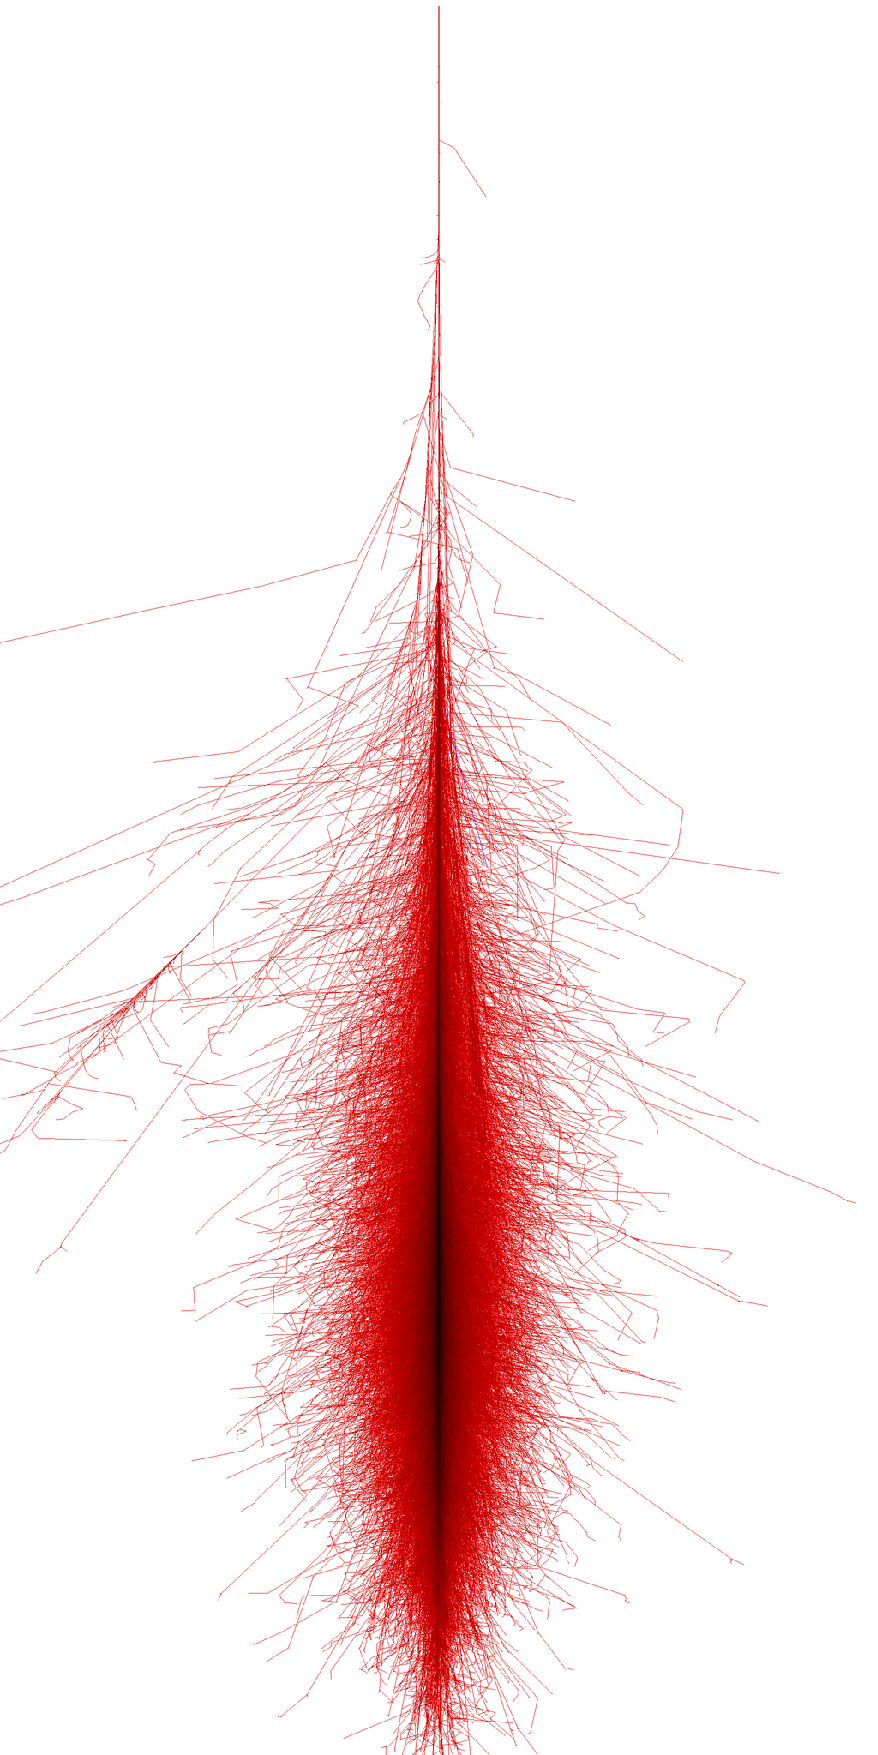
\includegraphics[width=\linewidth]{Pictures/photon_12_0deg.pdf}
  \endminipage\hfill
  \minipage{0.33\textwidth}
  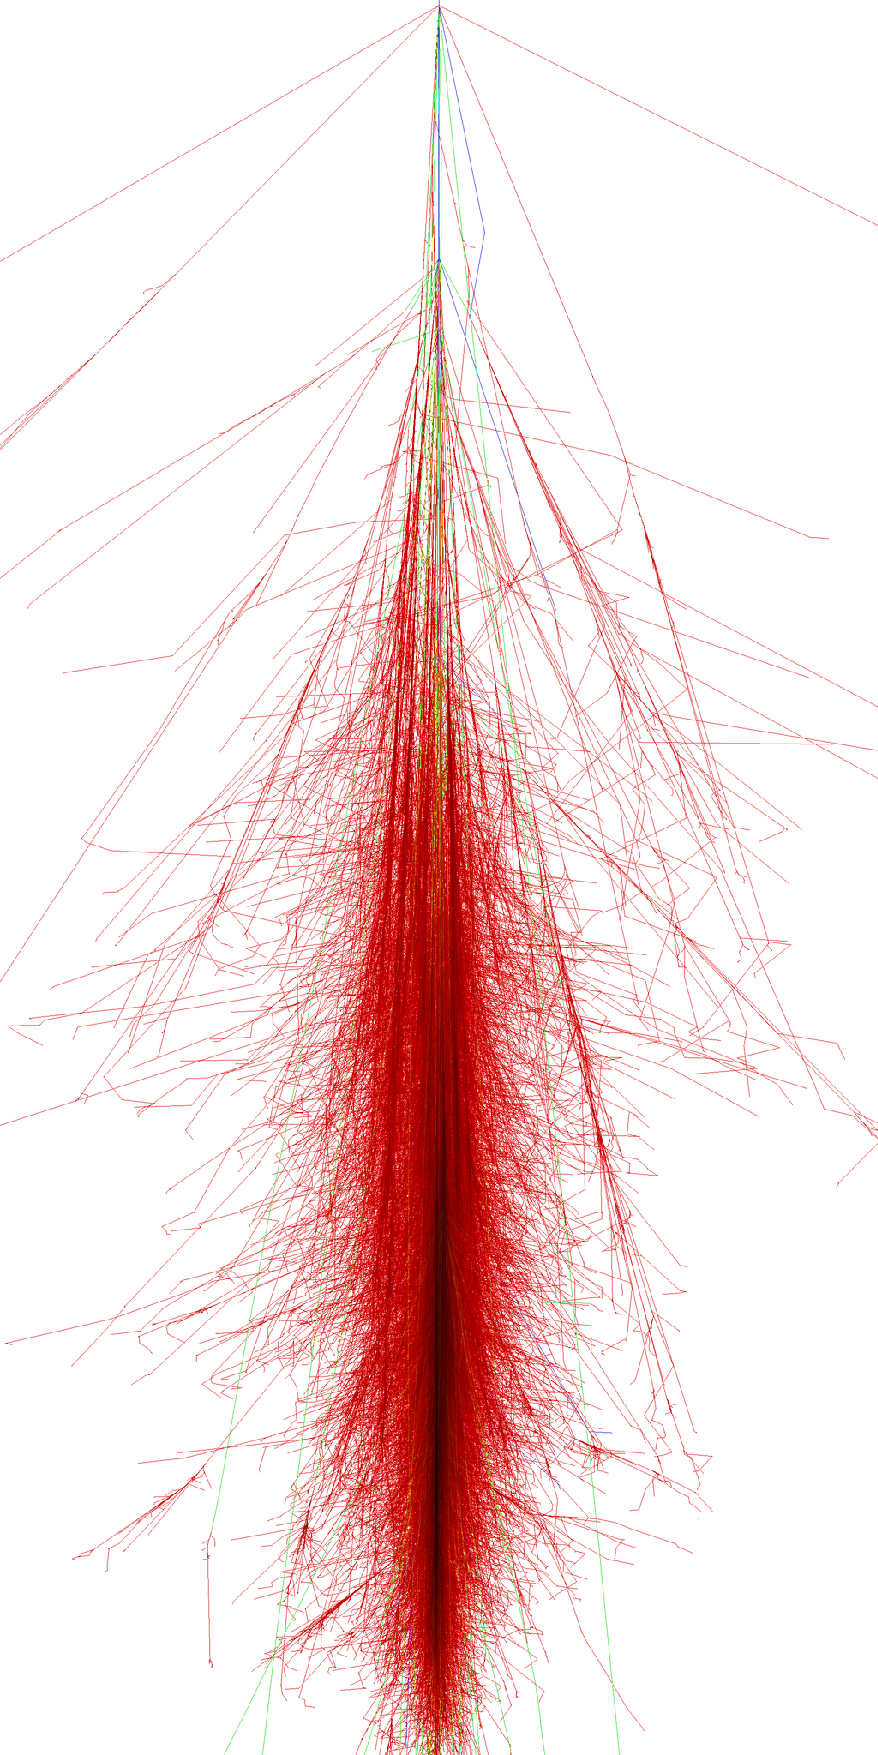
\includegraphics[width=\linewidth]{Pictures/proton_12_0deg.pdf}
  \endminipage\hfill
    \minipage{0.33\textwidth}
  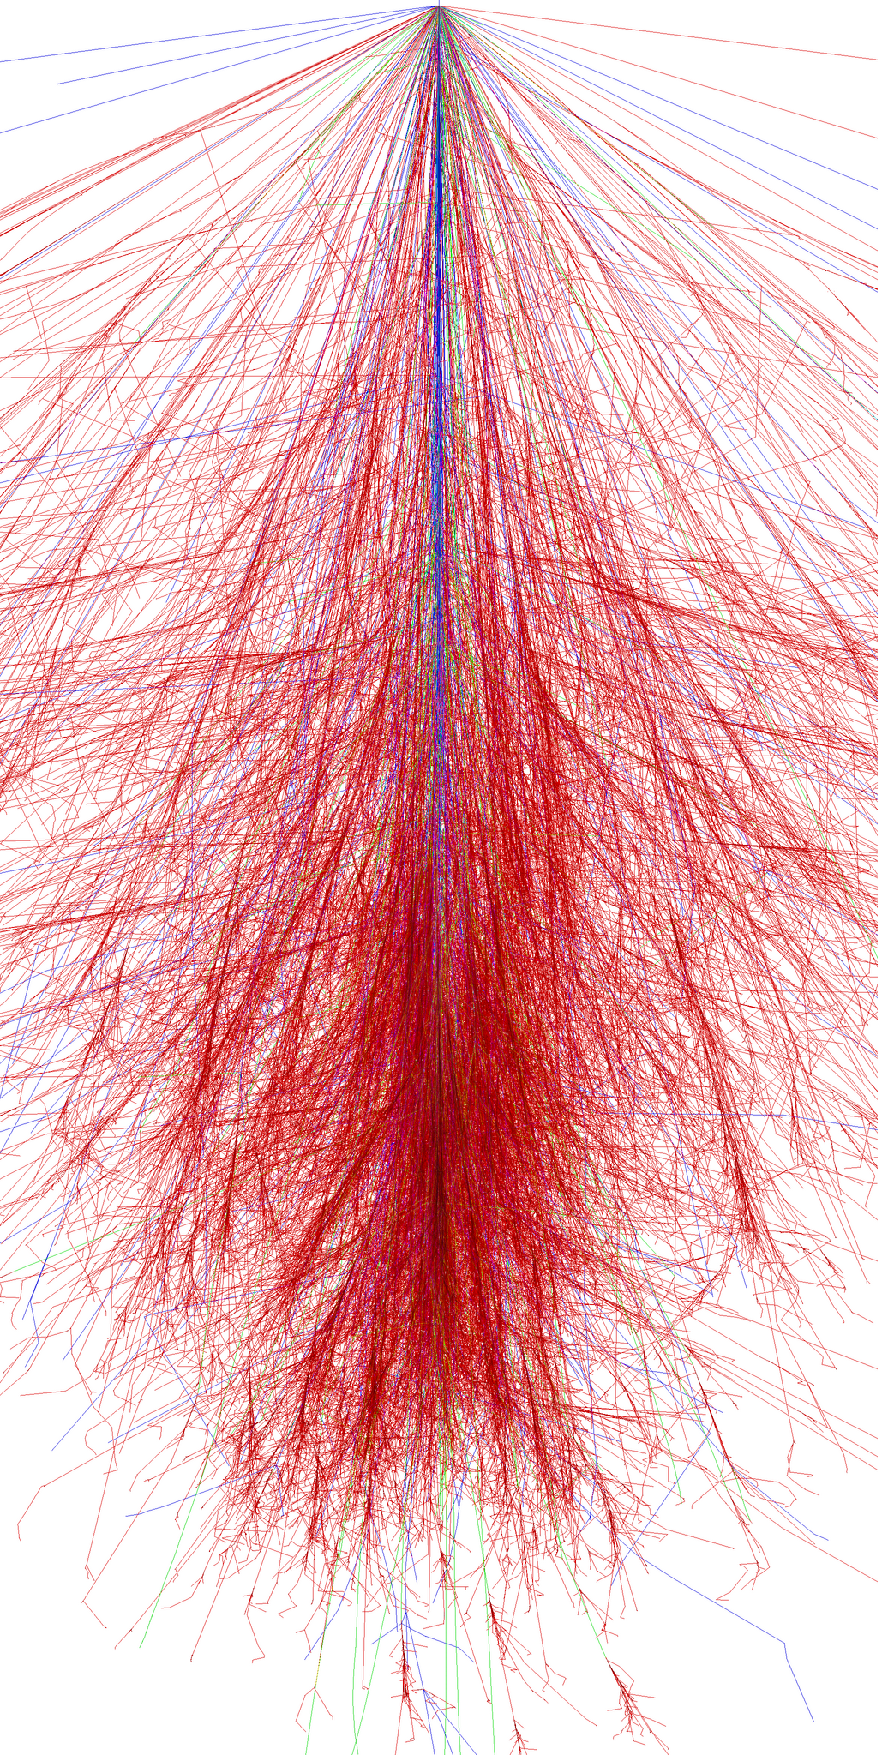
\includegraphics[width=\linewidth]{Pictures/iron_12_0deg.pdf}
  \endminipage\hfill
  \caption{\label{fig:corsika} Photon (left), proton (center) and iron (right) produced showers for a primary energy of 1 TeV and 0º zenith angle, simulated with \gls{corsika} from \cite{corsikaimages}.}
\end{figure}

\subsubsection{sim\_telarray}

The second part of \gls{mc} simulations is carried out by the program sim\_telarray \cite{2008corsikanadsimtelarray}, dedicated to the simulations of the detectors: Optical ray-tracing of photons, their registration by \glspl{pmt}, the behaviour of discriminators or comparators for trigger at pixel and telescope levels, and the digitalization of resulting signals. It was originally created for the \gls{hegra} \gls{iact} system, and has been improved and made fully configurable to be used with any kind of \gls{iact} layouts.\\
The simulation of ray-tracing follows the trajectory of photons since they reach the mirrors of the telescopes and arrive to the camera pixels. The mirror optics are simulated taking into account the configured mirror morphologies, dish shapes and segmentation. The shadowing of the camera structure can be also included in the simulation. The final step of ray-tracing simulation is the angular acceptance of the pixels, which usually are equipped with Winston cones (lightguides) to avoid gaps between neighbouring pixels. From ray-tracing simulations, the \gls{psf} of the telescopes can be calculated and hence can be used to optimize their designs. In the simulation of the photon detection by the \glspl{pmt}, the fluctuations in quantum efficiency in each pixel are taken into account.  As pixels are permanently exposed to \gls{nsb}, the number of photons arriving to each pixel is fully configurable assuming a specific \gls{nsb} spectrum. In the final simulation, the amplitude of the \gls{nsb} signal is subtracted from the signal baseline. The afterpulsing produced by ions is also taken into account, which is produced by ions hitting the photo-cathode, and can produce pulses of large amplitude which enter in the readout window of the front-end electronics of the cameras. The trigger system simulation takes into account the switching behaviour of discriminators or comparators, which can be configured to a specific logic (next-neighbour, pixel sectors...). The result from the pixel trigger system serves as input for the stereo level trigger, which usually requires that at least two telescopes trigger within a short time window. The final output of the sim\_telarray simulation is a data container in a format as closest as possible as the real data format from the actual instruments, based on the \textit{eventio} machine-independent format.

\subsection{Low level analysis: ctapipe} \label{sec:ctapipe}
The analysis of \gls{cta} data, both real and simulated, goes through different steps before turning into a format with which real science can be done. A description of the different \gls{cta} data levels is given in table \ref{tab:CTAdatalevels}. 


\begin{table}
  \centering
  \begin{tabular}{|l|l|}
    \hline
    Data level & Description \\
    \hline
    R0 & Raw data from camera, or \gls{mc} data\\
    R1 & Calibrated data \\
    DL0 & Data Volume Reduced Data \\
    DL1 & Calibrated image with Hillas parameters \\
    DL2 & Reconstructed shower parameters (Energy, direction and $\gamma$-hadron separation) \\
    DL3 & Reduced data, sets of gamma-like events with associated \gls{irf} and technical data\\
    & needed for science analysis \\
    DL4 & High level binned data products, like spectra, skymaps or light curves.\\
    DL5 & Legacy observatory data, like survey sky maps or source catalog. \\
    \hline
  \end{tabular}
  \caption{The different \gls{cta} data levels, based on \cite{ctapipe} and \cite{2015CTAdata}}
  \label{tab:CTAdatalevels}
\end{table}

\textit{Ctapipe} \cite{ctapipe} is a framework for prototyping the low-level data processing algorithms for \gls{cta}. It is written in Python and its currently in development, still suffering large and rapid changes to structure and functionality. While is not yet the final code for \gls{cta} analysis, and other alternatives are currently on development, \textit{ctapipe} is the framework chosen for the low level data analysis carried on in this thesis and so it is the one that will be described in this section.\\
The goal of \textit{ctapipe} is to reduce R0 data, that is raw data directly out of telescope cameras or \gls{mc} simulated data out from sim\_telarray, to DL2 data containing the reconstructed shower parameters.\\
Raw data can be read with \textit{ctapipe} thanks to specific \textit{EventSource} clases, which depend on the type of the input file (simulated data, real data from each specific telescope, etc.). It is possible to loop over the events of the source container to perform different operations on them. The first part of the data analysis is typically the calibration of the signal, requiring the treatment of the waveform signal in each pixel. \textit{Ctapipe} allows to perform the integration of the signal from the registered waveform using different types of integrators (\textit{LocalPeakWindowSum}, \textit{FullWaveformSum}...) to calculate the total number of counts in the pixel and transform it to number of photoelectrons. The result is a camera image, where pixels contain the light from the shower and from background. Different cleaning methods, like to two-level tailcuts cleaning, can be applied to subtract the background light and get the shower image. Afterwards, the Hillas parameters can be calculated. Other function allows to compute a linear fit to the extracted charge arrival times projected along the longitudinal axis of the Hillas ellipse, to extract the timing parameters. All these shower parameters are stored in the DL1 format, with the possibility to lose pixel-wise information and reduce the size of data files. For the reconstruction of the primary parameters, that is the energy, direction and particle type, there are currently two different algorithms implemented: A moment-based stereo reconstruction, which combines the Hillas parameters of different triggered telescopes geometrically to estimate the shower direction; and a template-based stereo reconstruction, which uses a fit of the full camera image to an expected image model to find the best fit shower axis, energy and depth of maximum. Other methods using machine learning and deep learning techniques are also being explored but are not yet implemented in the main source code of \textit{ctapipe.}\\


\subsection{Science analysis: ctools}

One of the proposed software packages for the scientific analysis of \gls{cta} data is \textit{ctools}, based on \textit{GammaLib} \cite{2016ctools}, a versatile toolbox for the scientific analysis of astronomical $\gamma$-ray data. It comprises a set of tools and python scripts with a command-line interface which allows interactive data analysis. It is possible also to create scripts and pipelines within Python using \textit{ctools} functionalities. The data managed by \textit{ctools} is at the level of DL3 and beyond, treating with observation events, skymaps, spectra and so on. For the analysis of observation events, \textit{ctools} includes the possibility of doing a binned (separating the data in energy bins) or unbinned analysis, and also it can stack the data of several observations to be analyzed together. A likelihood fitting can be performed to fit data to a given emission model, retrieving the best fit parameters of spectral, spatial and time components of the model of each emission source. Besides, \textit{ctools} allow to perform simulations of observations, using a set of precomputed \glspl{irf}, to be used as \textit{mock data} for the calculations of prospects of the future performance of \gls{cta}. Some of the most important tools of \textit{ctools} that has been used in this thesis are: \\

\begin{itemize}
\item \textit{ctobssim}: This tool produces simulations of event lists using the instrument characteristics specified by a given \gls{irf} and an input model. The model is composed of the individual models of each $\gamma$-ray source in the target \gls{fov}. Each model has a spatial component, given by the geometry of the source (point source, disk, gaussian, spatial map...), a spectral model describing the flux (it can be specific functions like power law or log parabola, or an user made spectrum where the flux per each energy is given in a file), and a time model, describing the variability of the source with time. The model also should include an instrumental background model to simulate background events, which are misclassified proton events.
  As input, \textit{ctobssim} requires a pointing direction, radius of the simulation region, time interval, energy interval, an \gls{irf} and an input model. The result is an event list in fits format, which contains all the information of the observation in the header.
\item \textit{ctbin}: This tool creates a counts cube, with a certain number of energy bins, and fills it with events from an event list. It is possible to stack events from different observations in the same counts cube. The resulting cube can be used in further steps of the analysis, like the likelihood fitting.
\item \textit{ctlike}: Performs a maximum likelihood fitting of a model to binned or unbinned data. As input, it can take event lists or a count cube, and depending on the input it will perform a binned or unbinned likelihood fit. A joint likelihood fitting can be done for multiple observations, and the average response functions (exposure, \gls{psf} and background) can be precomputed using the tools \textit{ctexpcube}, \textit{ctpsfcube} and \textit{ctbkgcube}. It is also possible to calculate the \gls{ts} (which is a measure of the source significance) of a source. More details on the likelihood fitting with \textit{ctools} will be given in chapter \ref{cap:LMC}.
\item \textit{ctmodel}: This tool generates 3-D model cube which provides the number of predicted number of counts for an input model as a function of spatial coordinates and energy. As an input, it will require a counts cube, an event list or an observation definition file and it will need the definition parameters of the cube, such as sky coordinates, projection, energy binning, number of pixels and pixel scale.
\item \textit{ctulimit}: Computes the upper flux limit for a specific source model. Starting from the maximum likelihood parameters, the tool will look for the flux that produces a decrease in the likelihood which corresponds to a given confidence level. By default, it is set at 95\% confidence level, but it can be configured. The result is the differential flux upper limit for a specified reference energy and the integrated flux in a certain energy range.
  
\end{itemize}



\end{document}
  
 
